\documentclass[a4paper, 12pt, oneside]{Thesis}  
\graphicspath{Figures/} 
\usepackage[square, numbers, comma, sort&compress]{natbib}
\usepackage{natbib}
\usepackage[nottoc,notlof,notlot]{tocbibind} 
\usepackage{subcaption}
\usepackage[utf8]{inputenc}
\usepackage{longtable}
\renewcommand\bibname{Bibliografie}
\renewcommand\contentsname{Cuprins}
\renewcommand\chaptername{Capitolul}
\usepackage{verbatim}  
\usepackage{vector}
\usepackage{graphicx}
\graphicspath{ {images/} }
\hypersetup{urlcolor=blue, colorlinks=true}

\begin{document}
\frontmatter     

\title  {Identificarea bolilor cardiace cu re\c{t}ele neuronale}
\authors  {\texorpdfstring
            {\href{daniel.lungu@my.fmi.unibuc.ro}{Lungu Daniel}}
            {Lungu Daniel}
            }
\addresses  {\groupname\\\deptname\\\univname}
\date       {\today}
\subject    {}
\keywords   {}
\maketitle
\setstretch{1.3}  
\fancyhead{}
\rhead{\thepage}
\lhead{}
\pagestyle{fancy}
\clearpage

\pagestyle{fancy}
\cfoot{\thepage}
\lhead{\emph{Identificarea bolilor cardiace cu re\c{t}ele neuronale}}
\rhead{}
\tableofcontents 
\mainmatter	  
\pagestyle{fancy}
\chapter{Inroducere}

\section{Inima}

Inima este motorul organismului, organul care ne \c{t}ine \^{i}n via\c{t}\u{a}. Aceasta are rolul de a prelua s\^{a}ngele \^{i}nc\u{a}rcat cu oxigen \c{s}i substan\c{t}e nutritive venite de la plam\^{a}n \c{s}i de al pompa spre toate celelalte organe prin aorta si arterele care se desprind din ea. De asemenea tot inima este cea care prime\c{s}te s\^{a}ngele inc\u{a}rcat cu dioxid de carbon de la toate organele prin sistemul venos \c{s}i il pompeaz\u{a} spre pl\u{a}m\^{a}ni pentru oxigenare. Acest circuit se repet\u{a} pe tot parcursul vie\c{t}ii far\u{a} a se \^{i}ntrerupe , p\^{a}n\u{a} c\^{a}nd \^{i}nceteaz\u{a} s\u{a} mai bat\u{a} \c{s}i murim ...
\par 
Bolile de inim\u{a} sunt principala cauz\u{a} de deces la nivel mondial, acestea curm\^{a}nd via\c{t}a unui numar mare de persoane. Potrivit medicilor speciali\c{s}ti num\u{a}rul mare de decese cauzate de bolile cardiovasculare se afl\u{a} \^{i}n direct\u{a} legetur\u{a} cu dificultatea identific\u{a}rii simptomelor deoarece nu sunt \^{i}ntotdeauna evidente \c{s}i de cele mai multe ori sunt ignorate sau atribuite unei altei afec\c{t}iuni.
\par 
Din fericire, progresul tehnologic din ultimii ani ne-a adus posibilitatea de a crea noi metode mai eficiente de identificare a simptomelor bolilor cardiace, astfel \^{i}nc\^{a}t acestea s\u{a} pot fi tratate \^{i}nc\u{a} de la apari\c{t}ia lor. O astfel de metod\u{a}, care presupune identificarea bolilor cardiace folosind \^{i}nregistrarile RMN (Rezonan\c{t}\u{a} Magnetic\u{a} Nuclear\u{a}) a unei persoane, preprocesarea lor \c{s}i utilizarea unei re\c{t}ele neuronale pentru stabilirea faptului dac\u{a} persoana respectiv\u{a} prezint\u{a} simptome ale bolilor cardiace, va fi prezentat\u{a} \^{i}n paginile de mai jos. 

\section{Imaginea}

TODO

\subsection{Rezonan\c{t}\u{a} Magnetic\u{a} Nuclear\u{a}}

Rezonan\c{t}a Magnetic\u{a} Nuclear\u{a} se folose\c{s}te de un c\^{a}mp magnetic \c{s}i de unde de radiofrecven\c{t}\u{a} pentru vizualizarea diferitelor organe \c{s}i \c{t}esuturi ale corpului omenesc. Undele de radiofrecven\c{t}\u{a} sunt apoi traduse \^{i}ntr-o imagine.

\section{Re\c{t}elele neuronale}

Re\c{t}elele Neuronale au pornit de la ideea de a crea un model matematic care s\u{a} imite structura \c{s}i comportamentul unui creier uman.
\par
Creierul este compus din mai multe unit\u{a}\c{t}i numi\c{t}i neuroni, care comunic\u{a} \^{i}ntre ei prin sinapse, se aproximeaz\u{a} faptul c\u{a} creierul uman are aproximativ 86 de miliarde de neuroni \c{s}i 10^{14} - 10^{15}  sinapse.


\includegraphics[width=300]{neuron_small.png}

Fiecare neuron prime\c{s}te impulsuri prin dedridele sale de la al\c{t}i neuroni \c{s}i produce impulsuri prin axon pe care il transmite mai departe la al\c{t}i neuroni prin sinapse.

\par

Acest model biologic a incercat sa fie imitat de c\u{a}tre Warren McCulloch \c{s}i Walter Pitts \^{i}n anul 1943, astfle \^{i}ncat ace\c{s}tia au creat un model matematic care s\u{a} semene c\^{a}t mai mult cu varianta biologic\u{a}. \^{I}n modelul matematic propus de ace\c{s}tia datele de intrare primite prin dendrive ( s\u{a} le not\u{a}m cu \textbf{\textit{x}} ) sunt multiplicate cu ni\c{s}te \^{i}nt\u{a}riri ( s\u{a} le not\u{a}m cu \textbf{\textit{w}} ) pentru a se imita transferul facut prin sinapse \^{i}ntre axonul neuronului care transmite datle \c{s}i dendrivele neuronului care prime\c{s}te datele. Corpul neuronului a devenit un sumator care \^{i}nsumeaza produsul primit de la dendrive, astfel c\u{a} acesta se poate definii prin func\c{t}ia  $$ f = \sum_{i=1}^{n} x_i w_i $$ unde \textbf{\textit{n}} reprezinta numarul de dendrive. 
\chapter{Re\c{t}elele neuronale}

\section{Neuronul}

Re\c{t}elele Neuronale au pornit de la ideea de a crea un model matematic care s\u{a} imite structura \c{s}i comportamentul unui creier uman.
\par
Creierul este compus din mai multe unit\u{a}\c{t}i numi\c{t}i neuroni, care comunic\u{a} \^{i}ntre ei prin sinapse, se aproximeaz\u{a} faptul c\u{a} creierul uman are aproximativ 86 de miliarde de neuroni \c{s}i 10^{14} - 10^{15}  sinapse.


\includegraphics[width=300]{neuron_small.png}

Fiecare neuron prime\c{s}te impulsuri prin dedridele sale de la al\c{t}i neuroni \c{s}i produce impulsuri prin axon pe care il transmite mai departe la al\c{t}i neuroni prin sinapse.

\par

Acest model biologic a incercat sa fie imitat de c\u{a}tre Warren McCulloch \c{s}i Walter Pitts \^{i}n anul 1943, astfle \^{i}ncat ace\c{s}tia au creat un model matematic care s\u{a} semene c\^{a}t mai mult cu varianta biologic\u{a}. \^{I}n modelul matematic propus de ace\c{s}tia datele de intrare primite prin dendrive ( s\u{a} le not\u{a}m cu \textbf{\textit{x}} ) sunt multiplicate cu ni\c{s}te \^{i}nt\u{a}riri ( s\u{a} le not\u{a}m cu \textbf{\textit{W}} ) pentru a se imita transferul facut prin sinapse \^{i}ntre axonul neuronului care transmite datle \c{s}i dendrivele neuronului care prime\c{s}te datele. Corpul neuronului a devenit un sumator care \^{i}nsumeaza produsul primit de la dendrive, astfel c\u{a} acesta se poate definii prin urm\u{a}toarea formul\u{a}  $$ \sum_{i=1}^{n} W_i x_i $$ unde \textbf{\textit{n}} reprezint\u{a} num\u{a}rul de dendrive. La aceast\u{a} formul\u{a} se mai insumeaz\u{a} un \textit{biases} ( s\u{a} \^{i}l not\u{a}m cu \textbf{\textit{b}} ) pentru a reprezenta caracteristicile neliniare ale neuronului. Cu aceast\u{a} nou\u{a} \^{i}nsumare formula va devenii $$ \sum_{i=1}^{n} W_i x_i + b $$
Dac\u{a} rezultatul ob\c{t}inut este mai mare dec\^{a}t un prag acesta va trece mai departe prin axon spre al\c{t}i neuroni. S\u{a} definim acest efect printr-o func\c{t}ie \textbf{\textit{f}} pe care o vom numii \textit{func\c{t}ie de activare} care stabile\c{s}te dac\u{a} un semnal trece mai departe sau nu, vom descrie mai pe larg aceast\u{a} func\c{t}ie in capitolele de mai jos, astfel c\u{a} modelul matematic a neuronului se poate rezuma la urm\u{a}toarea formul\u{a} 
$$f( \sum_{i=1}^{n} W_i x_i + b ) $$

\par

Trebuie precizat faptul c\u{a} modelul matematic al neuronului prezentat mai sus nici mac\u{a} nu se apropie de adevaratul comportament al unui neuron, acesta din urm\u{a} av\^{a}nd \^{i}n creierul uman un rol mult prea complex pentru a putea fi exprimat printr-o simpl\u{a} func\c{t}ie. 


\section{Fun\c{t}ia de activare}

A\c{s}a cum am specificat \c{s}i mai sus, o re\c{t}ea neuronala are nevoie de o fun\c{t}ie de activare care s\u{a} decid\u{a} dac\u{a} datele pot trece mai departe la urmatorii neuroni sau nu. De-a lungu istoriei s-au folosit mai multe tipuri de fun\c{t}ii de activare la re\c{t}elele neuronale, \^{i}nsa cea care d\u{a} cel mai bun randament at\^{a}t la timpul de antrenare c\^{a}t \c{s}i la acurate\c{t}ea final\u{a} este func\c{t}ia de activare ReLU (Rectified Linear Unit).

\subsection{Rectified Linear Unit}

Rectified Linear Unit, sau mai pe scurt ReLU, este la ora actual\u{a} cea mai folosit\u{a} fun\c{t}ie de activare, ea av\^{a}nd urm\u{a}toarea formul\u{a}

\[ f(x) =
  \begin{cases}
    0       & \quad \text{dac\u{a} } x \leq 0\\
    x  & \quad \text{dac\u{a} } x > 0\\
  \end{cases}
\]

Cu alte cuvinte func\c{t}ia pur \c{s}i simplu nu las\u{a} s\u{a} treac\u{a} mai departe rezultatele negative in urma efectu\u{a}rii opera\c{t}iilor din corpul neuronului.

\section{Arhitectura unei re\c{t}ele neuronale}

Acum c\u{a} am aflat ce este un neuron \c{s}i cum este simulat acesta din punct de vedere matematic trebuie s\u{a} discut\u{a}m cum sunt structura\c{t}i ace\c{s}tia \^{i}ntr-o re\c{t}ea neuronal\u{a}, pentru c\u{a} o re\c{t}ea nuronal\u{a} este compus\u{a} din milioane sau chiar sute de milioane de neuroni iar structurarea acestora este foarte important\u{a}.

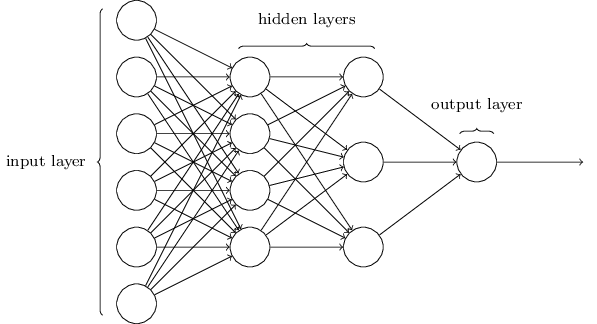
\includegraphics[width=300]{image10.png}

Re\c{t}elele neuronale sunt modelate ca o cole\c{t}ie de neuroni pe nivele, unde datele calculate de un nivel devin datele de intrare pentru urmatorul nivel de neuroni. Dupa cum se vede \c{s}i in imaginea de mai sus, neuronii afla\c{t}i pe acela\c{s}i nivel nu comunic\u{a} direct unii cu ceilal\c{t}i, comunicarea realiz\^{a}nduse doar cu nivelul inferior de neuroni \c{s}i cu nivelul superior de neuroni.
\par
Primul nivel al unei re\c{t}ele neuronale se nume\c{s}te nivelu input, deoarece acesta reprezint\u{a} doar date de intrare, iar ultimul nivel al unei re\c{t}ele neuronale se nume\c{s}te nivelul output, doarece acesta intoarce valoarea final\u{a}, nivelele dintre primul \c{s}i ultimul nivel se numesc nivelele ascunse ( hidden layers ).
\par
Re\c{t}elele neuronale, ca cea de mai sus, se numesc re\c{t}ele feedforward, deoarece outputul unui nivel merge tot timpul la urm\u{a}torul nivel, nu se intoarce niciodat\u{a} la un nivel anterior.
\par 
Pentru a se in\c{t}elege mai bine cum lucreaz\u{a} o re\c{t}ea neuronal\u{a} vom nota cu \textbf{\textit{x}} datele de intrare de la nivelul input, cu \textbf{\textit{h}} fiecare hidden layer, cu \textbf{\textit{W}} \^{i}ntaririle, cu \textbf{\textit{b}} bias-ul si cu \textbf{\textit{f}} func\c{t}ia de activare, astfle c\u{a} modelul de mai sus cu dou\u{a} niveluri hidden se poate exprima prin urm\u{a}torul algoritm:

$$h_1 = f( \sum_{i=1}^{n} W_1_i x_i + b_1 ) $$
$$h_2 = f( \sum_{i=1}^{n} W_2_i h_1_i + b_2 ) $$
$$out = f( \sum_{i=1}^{n} W_3_i h_2_i + b_3 ) $$

\par

Unul dintre motivele pentru care re\c{t}elele neuronale sunt organizate pe nivele este acela c\u{a} pe acest timp de structur\u{a} este mai u\c{s}or s\u{a} se efectueze opera\c{t}ii pe matrici, astfel inc\^{a}t sa nu mai fim nevoi\c{t}i s\u{a} facem multiplic\u{a}ri individuale. Spre exemplu, s\u{a} lu\u{a}m un \textbf{\textit{x}} de dimeniusne [10x10], $W_1, W_2 $ \c{s}i $W_3$ de dimensiune [5x10], [3x5], respectiv [1x3], iar $b_1, b_2 $ \c{s}i $b_3$ de dimensiune [5x1], [3x1] \c{s}i [1x1], atunci algoritmul de mai sus se poate rescrie in felul urmator: 

$$h_1 = f( W_1 x + b_1 ) $$
$$h_2 = f( W_2 h_1 + b_2 ) $$
$$out = f( W_3 h_2 + b_3 ) $$

unde $h_1$ este de dimensiune [5x10], $h_2$ de dimensiune [3x10], iar out de dimensiune [1x10]. Parametrii $W_1, W_2, W_3, b_1, b_2, b_3$ sunt paramterii pe care re\c{t}eaua neuronal\u{a} \^{i}i inva\c{t}\u{a} pentru a atinge o accurate\c{t}e c\^{a}t mai mare. Despre procesul de inv\u{a}\c{t}are a parametrilor \c{s}i despre cum trebuie s\u{a} \^{i}i set\u{a}m la inceput vom discuta \^{i}n capitolele ce urmeaz\u{a}.

\section{Initializarea parametrilor}

Am v\u{a}zut mai sus cum s\u{a} construim o re\c{t}ea neuronal\u{a}. \^{I}nainte ca s\u{a} discut\u{a}m descpre cum se antreneaz\u{a} o re\c{t}ea neuronal\u{a} trebuie s\u{a} discumta cum ini\c{t}ializ\u{a}m cele dou\u{a} tipuri de parametrii (\^{i}nt\u{a}ririle \c{s}i bias - urile). 

\subsection{Initializarea \^{i}nt\u{a}ririlor}

Av\^{a}nd in vedere c\u{a} nu \c{s}tiim valorile finale pe care o s\u{a} le aibe \^{i}nt\u{a}ririle la finalul procesului de antrenare a re\c{t}elei neuronale, deoarece aceste valori se actualizeaz\u{a} la fiecare pas de antrenare, va trebuii s\u{a} ini\c{t}ializ\u{a}m \^{i}nt\u{a}ririle astfle \^{i}nc\^{a}t o jum\u{a}tate din valori s\u{a} aibe valori negative iar cealalt\u{a} jum\u{a}tate valori pozitive, vom dorii valori unice pentru fiecare \^{i}ntarire pentru a acoperii o gam\u{a} c\^{a}t mai larg\u{a} de valori posibile pentru \^{i}nt\u{a}riri iar acestea s\u{a} fiu c\^{a}t mai aproape de valorea zero dar diferite de zero astfle \^{i}nc\^{a}t s\u{a} fiu mai u\c{s}or de actualizat.

\par

Pentru a \^{i}ndeplinii condi\c{t}iile de mai sus vom folosii o distribu\c{t}ie normal\u{a} cu media zero \c{s}i cu devia\c{t}ia standard $\frac{1}{\sqrt{n}}$ , unde n reprezint\u{a} numarul de variabile pe care \^{i}nt\u{a}rirea o are. Acest lucru asigur\u{a} faptul c\u{a} toate \^{i}nt\u{a}ririle din re\c{t}eaua neuronal\u{a} au la inceput aceea\c{s}i distribu\c{t}ie de numere, lucru care va facilita antrenarea mai rapid\u{a} a re\c{t}elei neuronale.

\par 

Dup\u{a} cum \c{s}tiim, varian\c{t}a reprezint\u{a} media patratic\u{a} a abaterilor in m\u{a}rime absolut\u{a} a valorilor inregistrare fat\u{a} de media aritmetic\u{a} care ne spune c\^{a}t de mare este r\u{a}sp\^{a}ndirea  acestui set. Mai precis, varian\c{t}a m\u{a}soar\u{a} c\^{a}t de apropiate sunt valorile setului de date de valoarea medie a acestuia.

$$Var = \frac{1}{n} \sum_{i=1}^{n} (x_i - m )^2 $$

\^{I}n formula de mai sus m reprezint\u{a} media aritmetic\u{a} iar $x_i$ valaorile date. \^{I}n cazul nostru dorim ca varian\c{t}a datelor de intrare sa nu se schimbe dup\u{a} ce iese din neuron \c{s}i se duce spre func\c{t}ia de activare pentru a nu altera datele foarte tare de la un nivel la altul. \^{I}n acest caz

$$Var(\sum_{i=1}^{n} W_i x_i) = \sum_{i=1}^{n} Var(W_i x_i) = $$
$$ = \sum_{i=1}^{n} [E(W_i)]^2 Var(x_i) + [E(x_i)]^2 Var(W_i) + Var(x_i) Var(W_i)$$

Presupunem c\u{a} setul de date \c{s}i \^{i}nt\u{a}ririle au media zero \c{s}i sunt distribuite identic, astfel c\u{a} formula de mai sus se transform\u{a} \^{i}n

$$\sum_{i=1}^{n} Var(x_i) Var(W_i) = (n Var(W)) Var(x)$$

care trebuie sa fie egal\u{a} cu varian\c{t}a datelor de intrare, asta \^{i}nseamn\u{a} c\u{a} 

$$n Var(W) = 1 \implies Var(W) =  \frac{1}{n} $$

\c{s}i \c{t}in\^{a}nd cont c\u{a} varian\c{t}a unei distribu\c{t}ii normale este p\u{a}tratul devia\c{t}iei standard, atunci rezult\u{a} c\u{a} devia\c{t}ia standard are valoarea $\frac{1}{\sqrt{n}}$ pentru distribu\c{t}ia normal\u{a} pe care o vom folosii pentru a alege valorile \^{i}nt\u{a}ririlor la ini\c{t}ializare.

\subsection{Initializarea bias}

Pentru bias-uri este comun de a le ini\c{t}ializa cu valorea zero sau cu o valoare foarte mic\u{a} apropiat\u{a} de zero, de exemplu 0.01. Din cauza faptului c\u{a} bias-ul nu joac\u{a} un rol a\c{s}a de important ca \^{i}nt\u{a}ririle \^{i}n re\c{t}eaua neuronal\u{a}, nu este de o importan\c{t}\u{a} foarte mare \^{i}n procesul de \^{i}nv\u{a}\c{t}are valoarea pe care o folosim la ini\c{t}ializarea lor, din acest motiv vom ini\c{t}ializa bias-ul cu valoarea zero.

\section{Procesul de antrenare}

Procesul de antrenare sau \^{i}nv\u{a}\c{t}are a unei re\c{t}ele neuronale const\u{a} din mai multe componente, prima component\u{a} se numeste func\c{t}ia de pierdere ( loss function \^{i}n englez\u{a} ) care penalizeaz\u{a} corectitudinea predic\c{t}iilor facute de c\u{a}tre re\c{t}eaua neuronal\u{a} fa\c{t}\u{a} de predic\c{t}iile corecte, a doua component\u{a} const\u{a} \^{i}n metode de prevenire a efectului de overfitting \^{i}n re\c{t}eaua neuronal\u{a}, a treia \c{s}i ultima component\u{a} este procesul de optimizare care actualizeaz\u{a} \^{i}nt\u{a}ririle si bias-urile din re\c{t}eaua neuronal\u{a} astfel \^{i}nc\^{a}t urmatoarele predic\c{t}ii ale re\c{t}elei neuronale s\u{a} fiu mai aproape de adev\u{a}r. \^{I}n continuare vom definii mai detaliat cele trei componente.

\subsection{Func\c{t}ia de pierdere}

Func\c{t}ia de pierdere are rolul de a m\u{a}sura compatibilitatea dintre predic\c{t}iile f\u{a}cute de c\u{a}tre re\c{t}eaua neuronal\u{a} \c{s}i valorile adev\u{a}rate. Aceast\u{a} func\c{t}ie face media \^{i}ntre rezultatele ob\c{t}inute de c\u{a}tre fiecare predic\c{t}ie \^{i}n urma aplicarii unei func\c{t}ii de cost care m\u{a}soar\u{a} c\^{a}t de aproape este predic\c{t}ia de adev\u{a}r.

$$L = \frac{1}{N} \sum_i L_i $$

Exist\u{a} mai multe variante de func\c{t}ii de cost \^{i}ns\u{a} cea mai folosit\u{a} \c{s}i cea mai eficient\u{a} la ora actual\u{a} este func\c{t}ia Softmax, care are urm\u{a}toarea formul\u{a}.

$$ L_i = - log \bigg(\frac{e^{f_y_i}}{\sum_j e^{f_j}}\bigg)$$

Unde $f_j$ reprezint\u{a} valoarea preconizat\u{a} de re\c{t}eaua neuronal\u{a} pentru clasa j, iar $f_y_i$ reprzint\u{a} valorea preconizat\u{a} pentru clasa corect\u{a}.

\par

Pentru a se \^{i}n\c{t}elege mai bine cum func\c{t}ioneaz\u{a} func\c{t}ia Softmax o s\u{a} d\u{a}m un mic exemplu. S\u{a} presupunem c\u{a} re\c{t}eaua neuronal\u{a} \^{i}ntoarce urm\u{a}torul set de date [5,−2,3] unde prima pozi\c{t}ie este valoarea pentru clasa corect\u{a}, astfel c\u{a} $f_y_i = 5$, atunci 

$$L_0 = - log \bigg(\frac{e^{5}}{e^{5} + e^{-2} + e^{3}} \bigg) = - log \bigg(\frac{148,413}{148,413 + 0,135 + 20,085}\bigg) =  $$
$$ = - log\bigg( \frac{148,413}{168,633} \bigg) = -log(0,88) = 0,055 $$

Func\c{t}ia Softmax penalizeaz\u{a} predic\c{t}iile re\c{t}elei neuronale ( calculeaz\u{a} o valoare mai mare ) atunci c\^{a}nd aceasta atribuie valori mari claselor incorecte iar valoarea calculat\u{a} este mai mic\u{a} atunci c\^{a}nd clasa corect\u{a} are o vloare atribuit\u{a} foarte mare fa\c{t}\u{a} de celelalte clase. A\c{s}a c\u{a} scopul principal al procesului de inv\u{a}\c{t}are este acela de a minimiza scorul pe care func\c{t}ia de pieredere \^{i}l calculeaz\u{a}, deoarece cu c\^{a}t func\c{t}ia de pierdere calculeaz\u{a} un scor mai mic cu at\^{a}t putem s\u{a} fim mai siguri ca re\c{t}eaua neuronal\u{a} a \^{i}nv\u{a}\c{t}at s\u{a} \^{i}ndeplineasc\u{a} mai bine sarcina pentru care a fost conceput\u{a}.

\subsection{Prevenirea efectului de overfitting}

Overtfitting apare c\^{a}nd o re\c{t}ea neuronal\u{a} are mai mul\c{t}i parametrii ( \^{i}ntariri \c{s}i bias - uri ) dec\^{a}t este necesar pentru a putea clasifica datele primite, astfel \^{i}nc\^{a}t re\c{t}eaua neuronal\u{a} \^{i}ncepe s\u{a} memoreze datele de antrenare \c{s}i nu mai \^{i}nva\c{t}\u{a} s\u{a} generalizeze, din aceast\u{a} cauz\u{a} atunci c\^{a}nd va trece la setul de date pentru care va trebuii s\u{a} fac\u{a} predic\c{t}ii / s\u{a} le clasifice va avea o acurate\c{t}e foarte mic\u{a} din cauz\u{a} c\u{a} nu a inv\u{a}\c{t}at nimic din setul de date de antrenare \c{s}i doar le-a memorat.

\par 

O bun\u{a} analogie cu efectul de overfitting este atunci c\^{a}nd un copil inva\c{t}\u{a} ce este o ma\c{s}in\u{a}, c\^{a}nd \^{i}i ar\u{a}t\u{a}m pentru prima dat\u{a} o ma\c{s}in\u{a} va \^{i}n\c{t}elege c\u{a} o ma\c{s}in\u{a} are patru ro\c{t}i, se poate deplasa, are u\c{s}i, geamuri, ins\u{a} dac\u{a} \^{i}i ar\u{a}t\u{a}m tot timpul acea\c{s}i ma\c{s}in\u{a} va crede faptul c\u{a} toate ma\c{s}inile au culoarea ro\c{s}ie, prin urmare orice obiect ro\c{s}u este o posibil\u{a} ma\c{s}in\u{a}, lucru care este total fals.

\par

O bun\u{a} metod\u{a} de a prevenii efectul de overfitting este de a aplica o fun\c{t}ie de regularizare la func\c{t}ia de pierdere astfel \^{i}nc\^{a}t s\u{a} penaliz\u{a}m \^{i}nt\u{a}ririle care au vlori mari deoarece \^{i}nt\u{a}ririle cu valori mari pot infleun\c{t}a  foarte mult predic\c{t}iile \c{s}i pot memora datele pe care ar trebuii s\u{a} le \^{i}nve\c{t}e de asemenea func\c{t}ia de regularizare trebuie s\u{a} favorizeze \^{i}nt\u{a}ririle cu date c\^{a}t mai dispersate posibil astfel \^{i}nc\^{a}t s\u{a} se generalizeze ceea ce \^{i}nva\c{t}\u{a} re\c{t}eaua neuronal\u{a} din setul de date de antrenare. O func\c{t}ie de regularizare care \^{i}ndepline\c{s}te aceste condi\c{t}ii este func\c{t}ia urm\u{a}toare:

$$ R(W) = \sum_i \sum_j W_{i,j}^2 $$

Pentru a dovedi faptul c\u{a} func\c{t}ia de mai sus \^{i}ndepline\c{s}te condi\c{t}iile dorite o s\u{a} d\u{a}m un mic exemplu, s\u{a} presupunem c\u{a} avem urm\u{a}torul set de date x = [1,1,1,1] \c{s}i \^{i}nt\u{a}ririle urm\u{a}toare $W_1 = [1,0,0,0], W_2 = [0.25, 0.25, 0.25, 0.25]$, ambele \^{i}nt\u{a}riri au acela\c{s}i produs matricial cu setul de date, $W^T_1 x = W^T_2 x = 1$, \^{i}ns\u{a} $R(W_1) = 1 $ \^{i}n timp ce $R(W_2) = 0.25$, dup\u{a} cum am zis deja scopul re\c{t}elei neuronale este acela de a minimiza func\c{t}ia de pierdere, din aceast\u{a} cauz\u{a} re\c{t}eaua neuronal\u{a} va prefera \^{i}nt\u{a}rirea $W_2$ \^{i}n locul \^{i}ntaririi $W_1$. Prin urmare func\c{t}ia de pierdere va avea forma urm\u{a}toare cu tot cu func\c{t}ia de regularizare :

$$L = \frac{1}{N} \sum_i - log \bigg(\frac{e^{W_y_i x_y_i}}{\sum_j e^{W_j x_j}}\bigg) + \lambda \sum_i \sum_j W_{i,j}^2 $$

$\lambda$ este un hiperparametru care poate fi reglat astfel \^{i}nc\^{a}t s\u{a} decidem c\^{a}t de mult s\u{a} influen\c{t}eze func\c{t}ia de regularizare procesul de \^{i}nv\u{a}\c{t}are.

\subsection{Procesul de optimizare}

Scopul procesului de optimizare este acela de a g\u{a}si  \^{i}nt\u{a}riri \c{s}i bias-uri care minimizeaz\u{a} func\c{t}ia de pierdere, acest proces este cel mai complicat dintre toate pentru c\u{a} trebuie calculat gradientul func\c{t}iei de pierdere care ne va spune in ce direc\c{t}ie trebuie actualizat \^{i}nt\u{a}ririle astfel \^{i}nc\^{a}t s\u{a} minimiz\u{a}m func\c{t}ia de pierdere.

\par 

Prin defini\c{t}ie gradientul este un c\^{a}mp vectorial ale c\u{a}rui componente sunt derivatele par\c{t}iale ale func\c{t}iei f \^{i}n raport cu o variabil\u{a} vecorial\u{a} $x = (x_1, x_2, ...., x_n)$, adic\u{a} :

$$\nabla f = \bigg( \frac{\delta f}{\delta x_1}, \frac{\delta f}{\delta x_2}, ... , \frac{\delta f}{\delta x_n}  \bigg)$$

Av\^{a}nd \^{i}n vedere faptul c\u{a} gradientul ne arat\u{a} direc\c{t}ia \^{i}n care func\c{t}ia are valorile cele mai mari vom dorii s\u{a} mergem \^{i}n direc\c{t}ia invers\u{a} ar\u{a}tat\u{a} de gardient deoarece scopul nostru este ca func\c{t}ia de pierdere s\u{a} aibe vloarea minim\u{a}. \^{I}ns\u{a} avem o problem\u{a} pentru c\u{a} gradientul ne zice direc\c{t}ia \^{i}n care s\u{a} mergem dar nu ne zice \c{s}i c\^{a}t s\u{a} mergem in aceea direc\c{t}ie din acest motiv ne putem trezii la un moment dat c\u{a} func\c{t}ia de pierdere \^{i}ncepe s\u{a} creasc\u{a} chiar dac\u{a} noi megem in direc\c{t}ia invers\u{a} spus\u{a} de gradient. O solu\c{t}ie la aceast\u{a} problem\u{a} este s\u{a} facem pa\c{s}i mici \^{i}n direc\c{t}ia invers\u{a} spus\u{a} de gradient, ace\c{s}ti pa\c{s}i se numesc rata de \^{i}nv\u{a}\c{t}are a re\c{t}elei neuronale, reprezent\^{a}nd cel mai important hiperparametru care trebuie setat manual dintr-o re\c{t}ea neuronal\u{a} deoarece dac\u{a} \^{i}l set\u{a}m prea mare nu vom ajunge niciodat\u{a} la punctul unde func\c{t}ia de pierdere are valoare minim\u{a}, iar dac\u{a} \^{i}l set\u{a}m prea mic o s\u{a} ajungem foarte greu la punctul de minim.

\par

\^{I}nainte s\u{a} calcul\u{a}m gradinetul func\c{t}iei noastre de pierdere vom introduce o variabil\u{a} intermediabil\u{a} p pentru a simplifica calculul

$$p_k = \frac{e^{f_k}}{\sum_j e^{f_j}}$$

Astfel c\u{a} func\c{t}ia Softmax devine

$$L_i = - log \big( p_{y_i} \big)$$

Iar derivata pentru aceasta este

$$\frac{\delta L_i}{\delta f_k } = p_k \quad c\^{a}nd \quad y_i \neq k$$

$$\frac{\delta L_i}{\delta f_k } = p_k - 1 \quad c\^{a}nd \quad y_i = k$$

O s\u{a} dam un mic exemplu pentru a se \^{i}n\c{t}elege mai bine cum se calculeaz\u{a} gradientul pe baza formulelor de mai sus, s\u{a} presupunem c\u{a} p a calculat urm\u{a}toarele valori p = [0.2, 0.3, 0.5] iar clasa corect\u{a} este cea din mijloc cu probabilitatea atribuit\u{a} de 0.3, cu ajutorul formulelor de mai sus gradientul va avea urm\u{a}toarile valori [0.2, -0.7, 0.5]. Av\^{a}nd \^{i}n vedere ce ne spune un gradient este destul de u\c{s}or de interpretat rezultatul ob\c{t}inut, acela c\u{a} trebuie s\u{a} cre\c{s}tem clasele incorecte cu 0.2 \c{s}i 0.5 pentru a avea un rezultat mai mare la func\c{t}ia de pierdere \c{s}i s\u{a} scadem clasa corect\u{a} cu -0.7, \^{i}ns\u{a} pentru ca noi dorim ca func\c{t}ia de pierdere s\u{a} calculeze un rezultat mai mic vom scade cele do\u{a} clase incorecte cu -0.2 \c{s}i -0.5 \c{s}i vom cre\c{s}te clasa corect\u{a} cu 0.7.

\par

Dup\u{a} calcularea gradientului func\c{t}iei de pierdere trebuie s\u{a} calcul\u{a}m gradientul pentru \^{i}nt\u{a}riri \c{s}i bias pentru a \c{s}tii \^{i}n ce direc\c{t}ie trebuie s\u{a} \^{i}i actualiz\u{a}m ca s\u{a} minimiz\u{a}m rezultatul func\c{t}iei de pieredere. Deja \c{s}tim gradientul func\c{t}iei de pierdere a\c{s}a c\u{a} este destul de u\c{s}or s\u{a} calcul\u{a}m gradientul pentru \^{i}nt\u{a}riri \c{s}i bias av\^{a}nd \^{i}n vedere faptul c\u{a} $f_k = W_k x_k + b_k$, prin urmare

$$\frac{\delta L_i}{\delta W_k} = \frac{\delta L_i}{\delta f_k} \frac{\delta f_k}{\delta W_k} = \frac{\delta L_i}{\delta f_k} x_k$$

$$\frac{\delta L_i}{\delta b_k} = \frac{\delta L_i}{\delta f_k} \frac{\delta f_k}{\delta b_k} = \frac{\delta L_i}{\delta f_k}$$

S\u{a} nu uitam faptul c\u{a} trebuie derivat\u{a} \c{s}i func\c{t}ia de regularizare care penalizeaz\u{a} \^{i}nt\u{a}ririle cu valori mari \c{s}i concentrare \^{i}ntr-un singur punct, astfel c\u{a} gradientul pentru \^{i}nt\u{a}riri devine 

$$\frac{\delta L_i}{\delta W_k} = \frac{\delta L_i}{\delta f_k} x_k + \frac{\delta R(W_k)}{\delt W_k} = \frac{\delta L_i}{\delta f_k} x_k + 2 \lambda W_k$$

Odat\u{a} calcula\c{t}i cei doi gradine\c{t}i putrem trece la pasul de actualizare a \^{i}ntaririlor \c{s}i bias - urilor 

$$ W_k = W_k + \zeta \frac{\delta L_i}{\delta W_k} $$
$$b_k = b_k + \zeta \frac{\delta L_i}{\delta b_k} $$

\^{I}n formulele de mai sus am notat cu $\zeta$ pasul de \^{i}nv\u{a}\c{t}are a re\c{t}elei neuronale. Acest tip de actualizare a parametrilor dintr-o re\c{t}ea neuronal\u{a} se nume\c{s}te SGD (Stochastic Gradient Descendent) care este destul de bun pentru o re\c{t}ea neuronal\u{a} simpl\u{a} cum avem noi acum, \^{i}ns\u{a} exist\u{a} varia\c{t}iuni ale acestei metode mult mai eficiente, cum ar fi Momentum de exemplu pe care o vom folosii la o re\c{t}ea neuronal\u{a} mult mai comlex\u{a} peste c\^{a}teva capitole.

\par

\^{I}n momentul de fa\c{t}\u{a} am actualizat doar ultimul nivel dintr-o re\c{t}ea neuronal\u{a}, \^{i}ns\u{a} ce facem dac\u{a} vrem s\u{a} actualiz\u{a}m parametrii de la nivelul inferior ei ? Cum putem calcula gradientul pentru ace\c{s}tia ? \^{I}nainte s\u{a} calculam gradentul pentru \^{i}nt\u{a}ririle si bias-urile de pe nivelul inferior trebuie s\u{a} calcul\u{a}m derivata func\c{t}iei de activare, reamintim faptul c\u{a} func\c{t}ia de activare are urmatoarea formul\u{a} 

\[ f(x) =
  \begin{cases}
    0       & \quad \text{dac\u{a} } x \leq 0\\
    x  & \quad \text{dac\u{a} } x > 0\\
  \end{cases}
\]

Calculul derivatei pentru func\c{t}ia de activare este necesar pentru c\u{a} aceasta ac\c{t}ioneaz\u{a} \^{i}ntre dou\u{a} nivele dintr-o re\c{t}ea neuronal\u{a} astfel c\u{a} dac\u{a} dorim s\u{a} actualiz\u{a}m parametrii unei re\c{t}ele neuronale de pe un nivel pe baza gradientului calculat de pe nivelul superior ei trebuie mai intai s\u{a} \^{i}l trecem prin derivate func\c{t}iei de activare, acest proces invers procesului normal pe care \^{i}l face o rec\c{t}ea neuronal\u{a} se mai nume\c{s}te \c{s}i backpropagation care are ca scop propagarea \^{i}napoi a gradinetului calculat la un pas superior.

\[ \frac{\delta f(x)}{\delta x}  =
  \begin{cases}
    0       & \quad \text{dac\u{a} } x \leq 0\\
    1  & \quad \text{dac\u{a} } x > 0\\
  \end{cases}
\]

Combinat\u{a} derivata de mai sus cu faptul c\u{a} aceasta las\u{a} doar valorile mai mari ca zero s\u{a} treac\u{a} mai departe va rezulta faptul c\u{a} aceasta va las\u{a} s\u{a} se propage \^{i}napo doar valorile de pe pozi\c{t}iile care au fost l\u{a}sate s\u{a} treac\u{a} \^{i}nainte la pasul normal.

\par

Acum c\u{a} am discutat teoretic toate elementele care alc\u{a}tuiesc o re\c{t}ea neuronal\u{a} standard e timpul s\u{a} le aplic\u{a}m peste problema noastr\u{a}, aceea de a identifica bolile cardiace la un pacient.

\section{Identificarea bolilor cardiace cu o re\c{t}ea neuronal\u{a} standard}
\chapter{Re\c{t}ele neuronale convolu\c{t}ionale}

Re\c{t}elele neuronale convolu\c{t}ionale  sunt foarte similare cu re\c{t}elele neuronale obi\c{s}nuite din capitolul anterior, ele sunt formate din neuroni care \^{i}nva\c{t}\u{a} \^{i}nt\u{a}riri \c{s}i bias-uri care s\u{a} \^{i}ndeplineasc\u{a} o anumit\u{a} sarcin\u{a}. Fiecare neuron prime\c{s}te date de intrare de la neuronii de pe nivelul inferior lor, efectuaz\u{a} o opera\c{t}ie de multiplicare \^{i}ntre \^{i}nt\u{a}riri \c{s}i datele de intrare, adun\u{a} bias-ul la rezultatul ob\c{t}inut \^{i}n urma multiplic\u{a}rii, iar dup\u{a}, de cele mai multe ori aplic\u{a} o func\c{t}ie de activare, iar la final dup\u{a} ultimul nivel aplic\u{a} o func\c{t}ie de cost care s\u{a} determine c\^{a}t de aproape este re\c{t}eaua neuronal\u{a} de adev\u{a}r \c{s}i dup\u{a} se aplic\u{a} propagarea \^{i}napoi pentru a actualiza \^{i}nt\u{a}ririle \c{s}i bias-ruile de pe fiecare nivel astfel \^{i}nc\^{a}t la urmatorul pas de \^{i}nv\u{a}\c{t}are a re\c{t}elei neuroanle aceasta s\u{a} ob\c{t}in\u{a} un rezultat mai mic de la func\c{t}ia de cost.

La prima vedere re\c{t}elele neuronale convolu\c{t}ionale seamana foarte mult cu re\c{t}elele neuronale obi\c{s}nuite, un lucru adevarat, \^{i}ns\u{a} exista unele diferen\c{t}e \^{i}ntre ele. Re\c{t}elele neuronale convolu\c{t}ionale pleac\u{a} de la prezum\c{t}ia c\u{a} datele de intrare de pe primul nivel sunt imagini, fa\c{t}\u{a} de re\c{t}elele neuronale obi\c{s}nuite, unde datele de intrare de pe primul nivel sunt ni\c{s}te vectori, din aceast\u{a} cauz\u{a} re\c{t}elele neuronale convolu\c{t}ionale se pot folosii de unele propiet\u{a}\c{t}i ale imaginilor, asfel \^{i}nc\^{a}t acestea s\u{a} fie mai eficiente in sarcini ce implica imaginile \c{s}i mai u\c{s}or de antrenat deoarece au nevoie de mai pu\c{t}ini parametrii dec\^{a}t ar avea nevoie o re\c{t}ea nuronal\u{a} obi\c{s}nuit\u{a} \^{i}n \^{i}ndeplinirea aceleia\c{s}i sarcini.

\section{Arhitectura unei re\c{t}ele neuronale convolu\c{t}ionale}

Cum am v\u{a}zut in capitolul anterior, re\c{t}elele neuronale obi\c{s}nuite primesc ca date de intrare un  vector pe care \^{i}l trec prin mai multe nivele de neuroni, unde fiecare neuron de pe un nivel este conectat cu to\c{t}i neuronii de pe nivelul urm\u{a}tor \c{s}i cu to\c{t}i neuronii de pe nivelul inferior lui, \^{i}ns\u{a} nu este conectat cu neuronii de pe acela\c{s} nivel cu el. 

\par

Faptul c\u{a} re\c{t}elele neuronale convolu\c{t}ionale sunt concepute special pentru sarcini ce implic\u{a} imagini \c{s}i c\u{a} datele de intrare  au trei dimensiuni ( l\u{a}\c{t}ime, \^{i}n\u{a}l\c{t}ime \c{s}i ad\^{a}ncime ),  fa\c{t}\u{a} de re\c{t}elele neuronale obi\c{s}nuite unde datele de intrare au o singur\u{a} dimensiune, neuronii de pe nivele trebuiesc rearanja\c{t}i astfel \^{i}nc\^{a}t s\u{a} \^{i}ndeplineasc\u{a} c\^{a}t mai bine sarcina pe care o au de f\u{a}cut \c{s}i s\u{a} se folosesc\u{a} c\^{a}t mai bine de propriet\u{a}\c{t}ile pe care le au imaginile. Din aceast\u{a} cauz\u{a} neuronii de pe un nivel la o re\c{t}ea neuronal\u{a} convolu\c{t}ional\u{a} sunt aranja\c{t}i pe trei dimensiuni ( l\u{a}\c{t}ime, \^{i}n\u{a}l\c{t}ime \c{s}i ad\^{a}ncime ), \^{i}n comapra\c{t}ie cu re\c{t}elele neuronale obi\c{s}nuite unde neuronii erau aranjati pe o singura dimensiune, cu acest timp de aranjament neuronii vor creea \^{i}nt\u{a}rir ce vor pune \^{i}n eviden\c{t}\u{a} anumite caracteristici ale unei imagine, caracteristici ce vor asigura o mai bun\u{a} performan\c{t}\u{a} a re\c{t}elei. Astfel c\u{a} un nivel dintr-o re\c{t}ea neuronal\u{a} convolu\c{t}ional\u{a} prime\c{s}te un volum de date cu trei dimensiuni \c{s}i produce un volum de date tot cu trei dimensiuni, volum de date care va fi dat mai departe la nivelul urm\u{a}tor lui.

\par 

\begin{center}
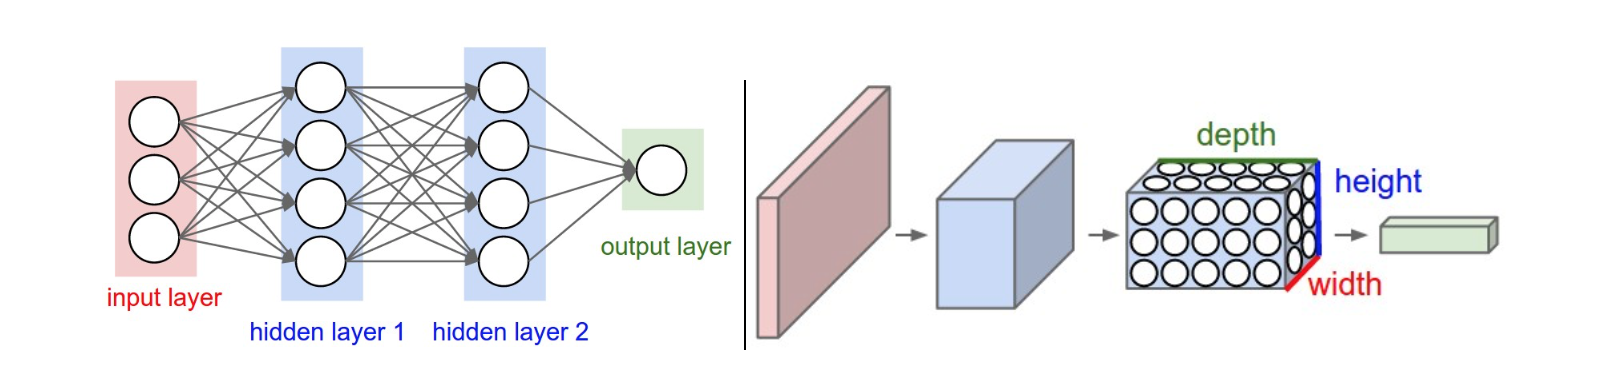
\includegraphics[width=450]{nn_cnn.png}
\end{center}

Imaginea de mai sus arat\u{a} diferen\c{t}a \^{i}ntre modul de aranjare a neuronilor pe o re\c{t}ea neuronal\u{a} obi\c{s}nuit\u{a} \c{s}i o re\c{t}ea neuronal\u{a} convolu\c{t}ional\u{a}.

\^{I}n re\c{t}elele neuronale convolu\c{t}ionale exit\u{a} trei tipuri de nivele, fa\c{t}\u{a} de re\c{t}elele neuronale obi\c{s}nuite unde exist\u{a} doar un singur tip, aceste nivele dintr-o re\c{t}ea neuronal\u{a} se numesc: nivelul convolu\c{t}ional, nivelul de pool \c{s}i nivelul conectat complet.

\subsection{Nivelul convolu\c{t}ional}

Nivelul convolu\c{t}ional este cel mai important nivel din cele trei \c{s}i cel care influen\c{t}eaz\u{a} cel mai mult deciziile re\c{t}elei neuronale. Acest nivel, ca \c{s}i nivelele din re\c{t}elele neuronale are doi paramterii, \^{i}nt\u{a}ririle \c{s}i bias-urile, ins\u{a} \^{i}nt\u{a}ririle sunt organizate pe trei dimensiuni cum am discutat mai sus, astfel \^{i}nc\^{a}t acestea s\u{a} devina ni\c{s}te filtre care \^{i}n urma aplic\u{a}rii lor asupra datelor de intrare s\u{a} scoat\u{a} \^{i}n eviden\c{t}u unele detalii descriminatorii care s\u{a} ajute la indeplinirea sarcinii, \^{i}ns\u{a} bias-urile sunt la fel ca la neuronii din re\c{t}elele neuronale obi\c{s}nuite. 

\par

De cele mai multe ori \^{i}nt\u{a}ririle sunt mici \^{i}n \^{i}n\u{a}l\c{t}ime \c{s}i l\u{a}\c{t}ime dar sunt foarte mari in ad\^{a}ncime. [3x3x512] este un exemplu de dimensiune a unei \^{i}nt\u{a}riri, unde \^{i}n\u{a}\c{t}imea \c{s}i l\u{a}\c{t}imea au dimensiune 3, iar ad\^{a}ncimea are dimensiunea 512, motivul pentru care ad\^{a}ncimea este a\c{s}a de mare, iar \^{i}n\u{a}l\c{t}imea \c{s}i l\u{a}\c{t}imea au dimensiuni a\c{s}a de mici  este pentru c\u{a} \^{i}n acest mod se pot construii mai multe filtre pe o por\c{t}iune mai mic\u{a} din datele de intrare \c{s}i, cum vom vedea in capitolele urm\u{a}toare, acest lucru faciliteaz\u{a} \^{i}n mod pozitiv acurate\c{t}ea re\c{t}elei neuronale.

\par

Nivelul convolu\c{t}ional gliseaz\u{a} o fereastr\u{a} de dimensiunea \^{i}nt\u{a}ririlor de-a lungul \c{s}i de-a latul datelor de intrare pornind de la col\c{t}ul de sus stanga a datelor de intrare \c{s}i face o \^{i}nmul\c{t}ire \^{i}ntre  datele de intrare aflate \^{i}n fereastr\u{a} \c{s}i cu \^{i}nt\u{a}ririle si  dup\u{a} la rezultat este adunat bias-ul. Acest proces este repetat p\^{a}n\u{a} c\^{a}nd fereastra ajunge in col\c{t}ul de jos dreapta a datelor de intrare. \^{I}n urma acestui proces va rezulta un volum de date bidimensional, dar acest proces este repetat pentru fiecare \^{i}nt\u{a}rire asftel c\u{a} la final vom avea un volum de date tridimensional. Cum am mai spus \c{s}i mai sus \^{i}nt\u{a}ririle \^{i}ntr-o re\c{t}ea neuronal\u{a} convolu\c{t}ional\u{a} sunt ni\c{s}te filtre care scot \^{i}n eviden\c{t}\u{a} anumte aspecte ale datelor de intrare, cum ar fi marginea unui obiect aflat \^{i}n imagine, o anumit\u{a} structur\u{a} care este caractersitic\u{a} unei anumite categorii de obiecte sau un patern.

\par

Pentru a se \^{i}n\c{t}elege mai bine cum func\c{t}ioneaz\u{a} nivelul convolu\c{t}ional s\u{a} presupunem c\u{a} avem o imagine de dimesniune [28x28x3] iar o \^{i}nt\u{a}rire are dimensiunea [5x5x3], a se observa faptul c\u{a} at\^{a}t  \^{i}nt\u{a}rirea c\^{a}t \c{s}i imaginea au aceea\c{s}i ad\^{a}ncime, respectiv 3, tot timpul ad\^{a}ncimea \^{i}nt\u{a}ririlor trebuie s\u{a} fie identic\u{a} cu cea a datelor de intrare pentru c\u{a} \^{i}n caz contrar nu s-ar putea face \^{i}nmul\c{t}irea \^{i}ntre datele de intrare \c{s}i \^{i}nt\u{a}riri, \^{i}ns\u{a} \^{i}n\u{a}l\c{t}imea si l\u{a}\c{t}imea \^{i}nt\u{a}ririlor trebuie s\u{a} fiu neap\u{a}rat mai mici dec\^{a}t a datelor de intrare astfel, nu s-ar putea face glisarea. Dimensiunea \^{i}nt\u{a}ririlor \^{i}n \^{i}n\u{a}l\c{t}ime \c{s}i l\u{a}\c{t}ime este setat\u{a} manual, fiind un parametru important de setat \^{i}ntr-o re\c{t}ea neuronal\u{a} convolu\c{t}ional\u{a}. 

\begin{center}
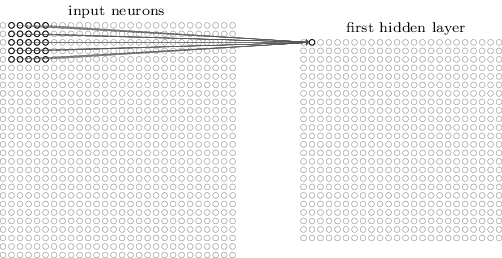
\includegraphics[width=300]{conv.png}
\end{center}

Cum se observ\u{a} \c{s}i \^{i}n imaginea de mai sus \^{i}n loc s\u{a} mai lu\u{a}m fiecare valoare a unui pixel separat \c{s}i s\u{a} o introducem \^{i}ntr-un neuron de pe un nivel intermediar ( hidden layer ) ca dat\u{a} de intrare putem s\u{a} grup\u{a}m pixelii in blocuri de pixeli \c{s}i s\u{a} \^{i}i trimitem grupa\c{t}i la un neuron de pe nivelul intermediar. \^{I}n cazul nostru vom face glisarea pe un grup de pixeli de dimensiunea [5x5x3] care va fi \^{i}nmul\c{t}it cu \^{i}nt\u{a}ririle noastre de dimensiune [5x5x3], \^{i}n urma rezultatului vom ob\c{t}ine o singur\u{a} valoare la care vom aduna bias-ul. Dac\u{a} se repeta procedeul  \c{s}i ne mi\c{s}c\u{a}m cu un pixel la dreapta, sau in jos pentru fiecare bloc de pixeli pe care vrem s\u{a} \^{i}l extragem, atunci ca rezultat vom avea [24x24x1] de valori. Acum s\u{a} presupunem c\u{a} avem 32 de astfel de \^{i}nt\u{a}riri pe acest nivel \c{s}i reptet\u{a}m procedeul pentru fiecare, atunci, ca rezultat final vom avea [24x24x32] de valori, valori care vor fi trimise mai departe c\u{a}tre urm\u{a}torul nivel. Un mare beneficiu al acestui mod de a grupa valorile \^{i}n blocuri de date mai mici, peste care s\u{a} efectu\u{a}m opera\c{t}ia de \^{i}nmul\c{t}ire \c{s}i de adunare este c\u{a} se reduce semnificativ numarul de valori la o  \^{i}nt\u{a}rire de care am fi avut nevoie dac\u{a} am fi f\u{a}cut acela\c{s} lucru pentru toate datele dintr-o dat\u{a}, cum se face \^{i}ntr-o re\c{t}ea neuronal\u{a} obi\c{s}nuit\u{a}, spre exemplu \^{i}n cazul exemplificat mai sus avem nevoie doar de 5 x 5 x 3 = 75 de valori pentru o \^{i}nt\u{a}rire, \^{i}n cazul unei re\c{t}ele neuronale obi\c{s}nuite am fi avut nevoie de 28 x 28 x 3 = 2352 de valori pentru o \^{i}nt\u{a}rire. Prin reducerea numarului de valori de care avem nevoie pentru o \^{i}nt\u{a}rire vom cre\c{s}te viteza de \^{i}nv\u{a}\c{t}are a re\c{t}elei neuronale \c{s}i vom putea cre\c{s}te complexitatea acesteia.

\par

Mai sus am discutat despre cum nivelul convolu\c{t}ional transform\u{a} un volum de date tridimensional \^{i}ntr-un alt volum de date tridimensional \c{s}i cum \^{i}l calculeaz\u{a} pe acesta, \^{i}ns\u{a} nu am discutat cum se calculeaz\u{a} dimensiunea volumului de date tridimensional rezultat \^{i}n urma aplicarii nivelului convolu\c{t}ional peste  datele de intrare. Sunt trei parametrii care controleaz\u{a} m\u{a}rimea datelor de ie\c{s}ire dintr-un nivel convolu\c{t}ional, acestea sunt: ad\^{a}ncimea, pasul de mi\c{s}care a ferestrei c\^{a}nd se face glisarea ei peste volumul de date \c{s}i padding-ul. Ad\^{a}ncimea corespunde numarului de \^{i}nt\u{a}riri pe care \^{i}l are respectivul nivel convolu\c{t}ional. Pasul este c\^{a}t de mult se mi\c{s}c\u{a} fereastra c\^{a}nd se face glisarea peste datele de intrare, dac\u{a} pasul este unu, atunci fereastra se va mi\c{s}ca la dreapta c\^{a}te un pixel, iar c\^{a}nd va ajunge la cap\u{a}t va combor\^{i} un pixel \c{s}i va merge din noul la dreapta c\^{a}te un pixel p\^{a}n\u{a} la cap\u{a}t, acest procedeu repet\^{a}ndu-se p\^{a}n\u{a} c\^{a}nd fereastra va ajunge \^{i}n col\c{t}ul de jos din dreapta. Dac\u{a} pasul este doi, atunci fereastra se va mi\c{s}ca doi pixeli la dreapta \c{s}i \^{i}n jos, \^{i}ns\u{a} acest lucru va produce mai pu\c{t}ine date de ie\c{s}ire dec\^{a}t dac\u{a} pasul era unu. Padding-ul presupune numarul de r\^{a}nduri cu valoare zero pe care le punem \^{i}n jurul datelor de intrare astfel \^{i}nc\^{a}t s\u{a} putem controla dimensiunea datelor de ie\c{s}ire. Spre exemplu cum aveam mai sus o imagine de dimesniune [28x28x3] \c{s}i \^{i}nt\u{a}riri de dimensiunea [5x5x3] \c{s}i un pas de unu aveam ca rezultat un volum de date de dimensiunea [24x24x1] pentru o \^{i}nt\u{a}rire, \^{i}ns\u{a} dac\u{a} ad\u{a}ug\u{a}m un padding de doi in jurul imaginii, atunci vom avea un volum de date de dimensiunea [32x32x3], deoarece padding-ul de doi s-a adugat jos, sus, la st\^{a}nga c\^{a}t \c{s}i la dreapta imaginii, iar \^{i}n urma aplic\u{a}rii nivelului convolu\c{t}ionale peste noul set de date vom avea un rezultat de dimensiunea [28x28x1]. Se observ\u{a} faptul c\u{a} noul rezultat are aceea\c{s}i dimensiune, at\^{a}t pe \^{i}n\u{a}l\c{t}ime, c\^{a}t \c{s}i pe l\u{a}\c{t}ime ca dimensiunea datelor ini\c{t}iale \^{i}nainte de aplicarea padding-ului, acest lucru,  de a pastra dimensiunea datelor de ie\c{s}ire egal cu cel al datelor de intrare pe \^{i}n\u{a}l\c{t}ime \c{s}i l\u{a}\c{t}ime este foarte des folosit \^{i}n practic\u{a}, deoarece prin acest fel se p\u{a}streaz\u{a} consisten\c{t}a datelor.

Putem s\u{a} exprim\u{a}m calculul volumului de ie\c{s}ire printr-o formul\u{a} foarte simpl\u{a} care arat\u{a} \^{i}n felul urm\u{a}tor:

$$ \frac{W - F + 2P }{S} + 1 $$

\^{I}n formula de mai sus, W este marimea volumui de date, F este m\u{a}rimea ferestrei prin care se face glisarea peste date, S este pasul de mi\c{s}care a ferestrei peste volumul de date, iar P este padding-ul care se adauga \^{i}n jurul volumului de date. Spre exemplu, dac\u{a} avem un volum de date de dimensiune 7x7 \c{s}i int\u{a}riri de dimensiunea 3x3 cu un pas de 1 si un padding de 0 atunci vom avea un rezultat de dimensiunea 5x5, \^{i}ns\u{a} dac\u{a} cre\c{s}tem pasul la 2 atunci vom avea un rezultat de dimensiunea 3x3.

\par

La o mic\u{a} analiz\u{a} se poate observa faptul c\u{a} pasul glis\u{a}rii ferestrei are anumite constr\^{a}ngeri, spre exemplu dac\u{a} volumul de date are o dimesniune de [10x10], padding-ul este 0 iar m\u{a}rimea ferestrei este de [3x3], atunci ar fi imposibil s\u{a} folosim un pas de 2, deoarece

$$ \frac{W - F + 2P }{S} + 1 = \frac{10 - 3 + 0 }{2} + 1 = 4.5 $$

\c{s}i av\^{a}nd \^{i}n vedere faptul c\u{a} dimensiunea datelor de ie\c{s}ire trebuie s\u{a} fie un num\u{a}r \^{i}ntreg atunci ar fi imposibil s\u{a} folosim un pas de 2 \^{i}ntr-un astfel de caz. \^{I}n astfel de cazuri dac\u{a} nu vrem s\u{a} schimb\u{a}m pasul, va trebuii s\u{a} adaug\u{a}m un padding \^{i}n jurul datelor de intrare astfel \^{i}nc\^{a}t s\u{a} ob\c{t}inem la final un num\u{a}r \^{i}ntreg ca dimensiune pentru volumul de date rezultat de c\u{a}tre nivelul convolu\c{t}ional, \^{i}n cazul nostru de mai sus dac\u{a} ad\u{a}ug\u{a}m un padding de 1, atunci vom avea  o dimensiune de [5x5] pentru volumul de date rezultat de c\u{a}tre nivelul convoli\c{t}ional.

\subsection{Niveulul de pool}

Nivelul de pooling se pune \^{i}ntre dou\u{a} nivele convolu\c{t}ionale pentru a se reduce cantitatea de informa\c{t}ie care se duce c\u{a}tre urm\u{a}torul nivel convolu\c{t}ional. Cel mai folosit tip de pooling este max-pooling care prime\c{s}te ca date de intrare valorile rezultate de la precedentul nivel convolu\c{t}ional \c{s}i le las\u{a} s\u{a} treac\u{a} doar pe cel cu valoarea cea mai mare c\u{a}tre urm\u{a}torul nivel convolu\c{t}ional ( vede\c{t}i imaginea de mai jos ), astfel c\u{a} acest nivel ne ajut\u{a} s\u{a} reducem cantitatea de date \c{s}i s\u{a} sc\u{a}p\u{a}m de datele nerelevante dintr-o re\c{t}ea convolu\c{t}ional\u{a}. 

\par

De cele mai multe ori nivelul max-pooling ia o fereastr\u{a} de dimensiune [2x2] \c{s}i o gliseaz\u{a} peste datele de intrare cu un pas de cu valoarea 2. La fiecare pas acest nivel ia valorile cuprinse \^{i}n fereastr\u{a} \c{s}i las\u{a} doar valoarea cea mai mare s\u{a} treac\u{a} mai departe, celelalte fiind eliminate. \^{I}n urma acestor opera\c{t}ii va fi redus\u{a} o catitate de 75\% din datele de intrare, spre exemplu dac\u{a} avem un volum de date de dimensiunea [32x32x32] \c{s}i aplic\u{a}m peste el un max-pool cu o fereastr\u{a} de dimensiunea [2x2] \c{s}i un pas de 2 atunci vom avea ca rezultat un volum de date de dinensiunea [16x16x32], de precizat faptul c\u{a} nivelul max-pool nu afecteaz\u{a} ad\^{a}ncimea datelor de intrare.

\begin{center}
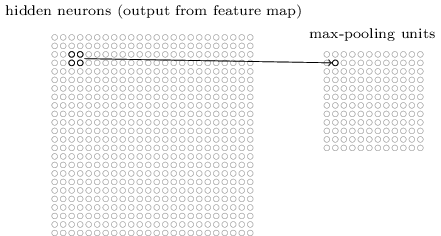
\includegraphics[width=300]{pool.png}
\end{center}

Cum se observ\u{a} \c{s}i \^{i}n imaginea de mai sus, nivelul de max-pooling prime\c{s}te patru valori de pe nivelul precedent \c{s}i las\u{a} o singur\u{a} valoarea s\u{a} treac\u{a} mai departe.

Un mare beneficiu pe care nivelul max-pool \^{i}l are asupra unei re\c{t}ele neuronale convolu\c{t}ionale este acela c\u{a} ne permite s\u{a} aplic\u{a}m nivele convolu\c{t}ionale mai mari peste date dup\u{a} ce am aplicat nivelul max-pool, acest lucru este posibil deoarece, cum am mai zis \c{s}i mai sus, nivelul max-pool ne scap\u{a} de o cantitate semnificativ\u{a} de date, prin urmare cantitate de date va fi mai mic\u{a} \c{s}i timpul de aplicare a unei \^{i}nt\u{a}riri va fi mai mic, prin urmare vom putea s\u{a} aplicam mai multe \^{i}nt\u{a}riri la urmatatorul nivel convolu\c{t}ional f\u{a}r\u{a} s\u{a} cre\c{s}tem timpul de calcul.

\subsection{Nivelul conectat complet}

Nivelul conectat complet este identic cu un nivel dintr-o re\c{t}ea neuronal\u{a} obi\c{s}nuit\u{a}, \^{i}n ideea c\u{a} fiecare neuron de pe nivelul inferior este conectat cu fiecare neuron de nivelul superior lui.

\par

Pentru a ad\u{a}uga un nivel conectat complet dup\u{a} un nivel convolu\c{t}ional, sau un nivel de pool, va trebuii s\u{a} redimension\u{a}m volumul de date trimidimensional care rezult\u{a} din astfel de nivele, pentru c\u{a}, nivelul conectat complet accept\u{a} ca date de intrare un volum de date unidimensional (vector). A\c{s}a c\u{a}, spre exemplu, atunci c\^{a}nd avem un volum de date rezultat dintr-un nivel convolu\c{t}ional de marimea, s\u{a} zicem, [7x7x512] va trebuii s\u{a} \^{i}l redimensionam la un vector cu 25088 de elemente, deoarece 7 x 7 x 512 = 25088, iar dup\u{a} aceea s\u{a} \^{i}numl\c{t}im datele redimensionate cu o \^{i}nt\u{a}rire de dimensiune, spre exemplu \^{i}n cazul pe care \^{i}l exemplific\u{a}m acum, [1024x25088] ,iar la rezultatul ob\c{t}inut \^{i}n umra \^{i}nmul\c{t}irii s\u{a} adun\u{a}m un bias, \^{i}n cazul nostru bias-ul  va avea 1024 de elemente.

\subsection{A\c{s}ezarea nivelelor}

Am v\u{a}zut p\^{a}n\u{a} acum c\u{a} re\c{t}elele neuronale convolu\c{t}ionale sun alc\u{a}tuite din trei tipuri de nivele (nivelul convolu\c{t}ional, nivelul de pool \c{s}i nivelul conectat complet). \^{I}n aceast\u{a} sec\c{t}iune vom discuta despre modalit\u{a}\c{t}ile de a a\c{s}eza aceste nivel \^{i}ntr-o re\c{t}ea neuronal\u{a} convolu\c{t}ional\u{a}.

\par

De cele mai multe ori o re\c{t}ea neuronal\u{a} convolu\c{t}ional\u{a} este alc\u{a}tuit\u{a} din mai multe nivele convolu\c{t}ionale, unde dup\u{a} fiecare nivel convolu\c{t}ional poate urma un nivel de pool, iar la final este ad\u{a}ugat unu sau mai multe nivele conectate complet unde ultimul nivel conectat complet va \^{i}ntoarce datele de ie\c{s}ire din re\c{t}eaua neuronal\u{a}. Cu alte cuvinte, de cele mai multe ori o re\c{t}ea neuronal\u{a} convolu\c{t}ional\u{a} respect\u{a} urm\u{a}torul tip de \c{s}ablon c\^{a}nd vine vorba de a\c{s}ezarea nivelelor :

\par

\text{Date de intrare} \longrightarrow [[\text{Nivel convolu\c{t}ional} \longrightarrow \text{ReLU}]*N \longrightarrow \\
\longrightarrow \text{Nivel pool ? } ] * M \longrightarrow [\text{Nivelul conectat complet} \longrightarrow \text{ReLU}] * K  \longrightarrow \\
\longrightarrow \text{Nivelul conectat complet} \longrightarrow \text{Date de ie\c{s}ire}

\^{I}n \c{s}ablonul de mai sus, stelu\c{t}a reprezint\u{a} de c\^{a}te ori se repet\u{a} secven\c{t}a de nivele din parantezele p\u{a}trate, iar N, M \c{s}i K reprezint\u{a} num\u{a}rul de repeti\c{t}ii, unde fiecarea valoare trebuie s\u{a} fie mai mare sau egal\u{a} cu zero. Am notat cu semnul \^{i}ntreb\u{a}rii nivelul pool doarece acesta poate ap\u{a}rea sau nu dup\u{a} nivelul convolu\c{t}ional.

\par

Un exemplu de astfle de re\c{t}ea neuronal\u{a} care s\u{a} respecte \c{s}ablonul de mai sus ar fi urm\u{a}toarea:

\text{Date de intrare} \longrightarrow \text{Nivel convolu\c{t}ional 1} \longrightarrow \text{ReLU} \longrightarrow \text{Nivel pool 1} \longrightarrow \\ 
\longrightarrow \text{Nivel convolu\c{t}ional 2} \longrightarrow \text{ReLU} \longrightarrow \text{Nivel pool 2} \longrightarrow \\ 
\longrightarrow  \text{Nivelul conectat complet} \longrightarrow \text{Date de ie\c{s}ire}

\^{I}n exemplul dat mai sus, N are valoarea 1, M are valoarea 2, iar K are valoarea 0.

\section{Prevenirea efectului de overfitting}

TODO

\subsection{Dropout}

TODO

\subsection{Batch Normalization}

TODO

\section{Procesul de antrenare}

A\c{s}a cum am precizat mai sus, la re\c{t}elele neuronale obi\c{s}nuite, procesul de antrenare const\u{a} \^{i}n actualizarea ponderilor \c{s}i bias-urilor dintr-o re\c{t}ea neuronal\u{a} cu o anumit\u{a} valoare, calculat\u{a} pe baza gradientului calculat \c{s}i \^{i}nmul\c{t}it\u{a} cu o constant\u{a}, care se nume\c{s}te rata de antrenare.

C\^{a}nd am discutat despre procesul de antrenare la re\c{t}ele neuronale obi\c{s}nuite am descris metoda SGD, \^{i}ns\u{a} a\c{s}a cum am preciza, SGD nu este suficent de eficent \c{s}i exist\u{a} alte metode mai eficinete de antrenare a unei re\c{t}ele neuronale. Metoda pe care o vom descrie mai jos, \c{s}i pe care o vom folosi \^{i}n procesul de antrenare a re\c{t}elelor neuronale convolu\c{t}ionale pe care le vom construii pentru a reozolva problema noastr\u{a}, se nume\c{s}te Adam.

\subsection{Adam}

Adam este o metod\u{a} nou\u{a} folisit\u{a} pentru actualizarea paramtetrilor dintr-o re\c{t}ea neuronal\u{a} obi\c{s}nuit\u{a}. Numele s\u{a}u deriveaz\u{a} din cuvintele adaptive moment estimation \c{s}i a fost inventat\u{a} de Diederik P. Kingma de la Universitatea din Amsterdam \c{s}i de Jimmy Lei Ba de la Universitatea din Toronto. Metoda propusa de ace\c{s}tia are urmatoarea formul\u{a}:

$$ m = \beta_1 \cdot m + ( 1 - \beta_1 ) \cdot \delta x $$
$$ v = \beta_2 \cdot v + ( 1- \beta_2 ) \cdot \delta x^2 $$
$$ x = x - \zeta \cdot \frac{m}{\sqrt{v} + \epsilon } $$

\^{I}n formulele de mai sus $\beta_1, \beta_2 $ \c{s}i $ \epsilon $ sunt trei constante pentru care autorii sugereaz\u{a} urmatoarele valor, $\beta_1 = 0.9 $, $\beta_2 = 0.999 $ \c{s}i $ \epsilon = 1e^{-8} $, vom pastra aceste valori \^{i}n re\c{t}elele noastre convolu\c{t}ionale. Valorile m \c{s}i v sunt la inceput ini\c{t}ializate cu valoarea zero, aceste valori, confomr autorilor, au rolul de a corecta anumite erori atunci c\^{a}nd se actualizeaz\u{a} parametrii re\c{t}elei. Cu $\zeta$ am notat rata de \^{i}mv\u{a}\c{t}are a re\c{t}elei neuronale.

\section{Procesarea datelor}

\^{I}nainte ca datele s\u{a} intre \^{i}ntr-o re\c{t}ea neuronal\u{a}, acestea trebuiesc preprocesate, astfle \^{i}nc\^{a} re\c{t}elei neuronale s\u{a} \^{i}i fie mai u\c{s}or s\u{a} \^{i}nve\c{t}e. Cele mai folosite metode de preprocesare a datelor sunt centrarea la origine a datelor \c{s}i normalizarea. Exist\u{a} o gramad\u{a} de metode de procesare a datelor, \^{i}ns\u{a} acestea sunt aplicabile doar pentru anumite seturi de date, \^{i}n timp ce, cele do\u{a} men\c{t}ionate mai sus sunt generale pentru orice tip de date \c{s}i pentru orice tip de re\c{t}ea neuronal\u{a}.

Pentru a exemplifica cum functioneaz\u{a} cele doua metode, vom presupune c\u{a} avem un set de date bidimensional ce are graficul urmator.

\begin{center}
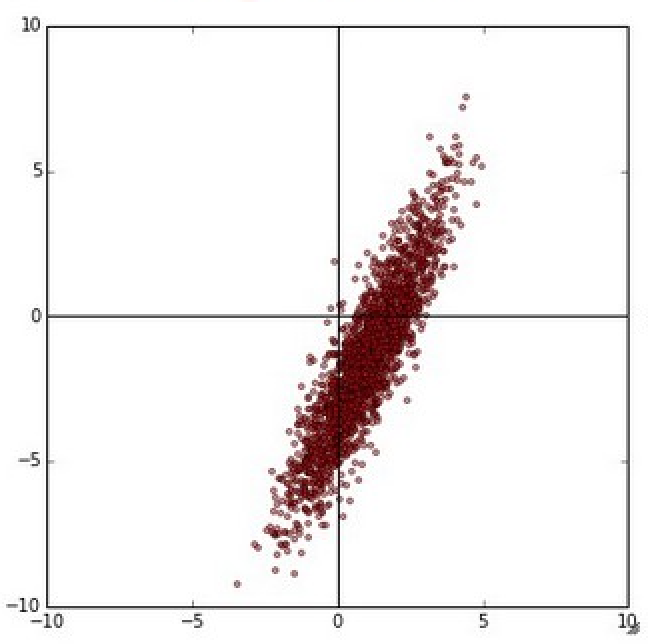
\includegraphics[width=200]{original.png}
\end{center}

Centrarea la origine a datelor, presupune ca pentru fiecare valorea s\u{a} sc\u{a}dem media valorilor din respectivul set de date.

            $$ X = X - \frac{1}{N}\sum_i^N X_i$$
            
Aceast\u{a} opera\c{t}ie va aduce centrul datelor la origine. \^{I}n cazul nostru de mai sus, dup\u{a} aplicarea opera\c{t}iei, graficul datelor va arata in felul urm\u{a}tor.

\begin{center}
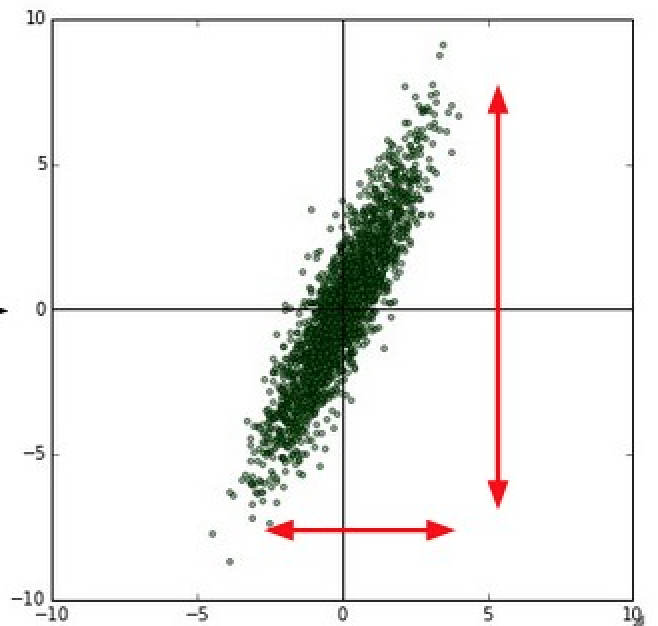
\includegraphics[width=200]{zero-centered.png}
\end{center}

Se observ\u{a} faptul c\u{a}, centrul datelor s-a mutat la origine.

Normalizarea datelor, presupune ca fiecare valoare din setul de date s\u{a} aibe acea\c{s}i scal\u{a}, modul de a efectua acest lucru este de a \^{i}mp\u{a}r\c{t}i fiecare valoare din setul de date cu devia\c{t}ia standard pe care o are setul de date. Dac\u{a} vom aplica aceast\u{a} opera\c{t}ie pe setul de date vom ob\c{t}ine urmatorul grafic.

\begin{center}
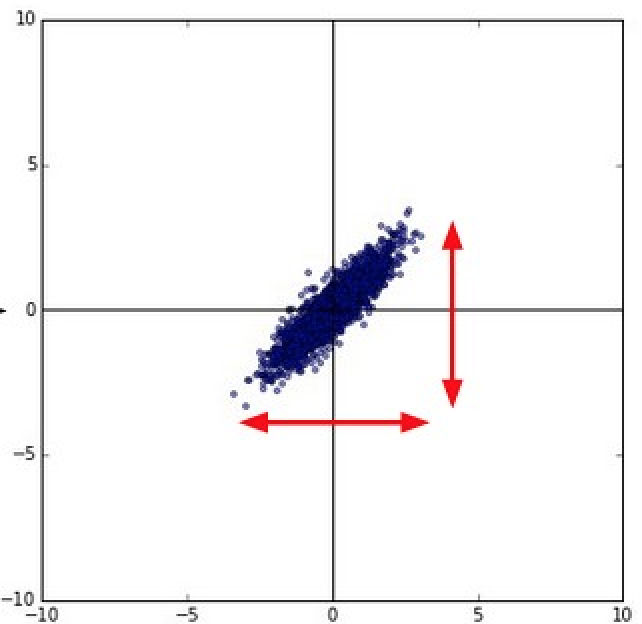
\includegraphics[width=200]{normalization.png}
\end{center}
\chapter{Identificarea bolilor cardiace cu re\c{t}ele neuronale}

\^{I}nainte s\u{a} aplic\u{a}m o re\c{t}ea neuronal\u{a} peste setul nostru de date trebuie mai \^{i}nt\^{a}i s\u{a} le preproces\u{a}m pentru a le converti la un format mai adecvat, s\u{a} elimin\u{a}m unele date nedorite din setul de date care pot \^{i}ngreuna procesul de antrenare \c{s}i s\u{a} ad\u{a}ug\u{a}m unele date care ne vor fi folositoare pe parcurs.

\section{Preprocesarea datelor}

Deoarece datele furnizate de c\u{a}tre The National Heart, Lung, and Blood Institute sunt in format DICOM (Digital Imaging and Communications in Medicine), format destul de greu de lucrat, prima noastr\u{a} sarcin\u{a} va fi s\u{a} le convertim la un format mult mai propice, cum ar fi formatul PNG (Portable Network Graphics), pentru a putea cre\c{s}te viteza de calcul a re\c{t}elei neuronale. \^{I}nainte de a le convertii de la format DICOM la PNG putem s\u{a} mai extragem unele informa\c{t}ii de la fiecare radiografie pe care formatul DICOM le ofer\u{a}, cum ar fi spre exemplu  id-ul pacientului caruia \^{i}i apar\c{t}ine radiografia, numarul de linii \c{s}i de coloane a radiografiei, care definesc marimea , spa\c{t}iul \^{i}ntre pixeli, care reprezint\u{a} o pereche de numere care arat\u{a} distan\c{t}a fizic\u{a} dintre centrii a doi pixeli pe vertical\u{a}, respectiv orizontal\u{a}, acestea fiind m\u{a}surate in milimetrii, ad\^{a}ncimea radiografiei masurat\u{a} in milimetrii, pozi\c{t}ia imaginii, care reprezint\u{a} coordonatele pe axele x, y \c{s}i z, fa\c{t}\u{a} de col\c{t}ul de sus st\^{a}nga al imaginii a centrului  radiografiei facute, loca\c{t}ia relativ\u{a} a radiografiei reprezentat\u{a} in milimetrii \c{s}i axa de codificare a imaginii (dac\u{a} e pe coloan\u{a} sau pe r\^{a}nd ). Toate aceste informa\c{t}ii ne vor fi folositoare pe parcurs a\c{s}a c\u{a} le vom salva \^{i}ntr-un fi\c{s}ier CSV.

\par

Dup\u{a} citirea imaginii vom verifica dac\u{a} imaginea este orientat\u{a} pe coloan\u{a}, \^{i}n acest caz dac\u{a} este adev\u{a}rat  va trebuii s\u{a} calcul\u{a}m transpusa imaginii (liniile vor deveni coloane) \c{s}i s\u{a} o rotim pe orizontal\u{a} de-a lungul axei x, astfel \^{i}nc\^{a}t sus s\u{a} devin\u{a} jos \c{s}i invers, jos s\u{a} devin\u{a} sus, astfel c\u{a} la final imaginea va fi rotit\u{a} cu 90 de grade, iar dintr-o imagine orientat\u{a} pe coloan\u{a} vom avea o imagine orientat\u{a} pe r\^{a}nd. Imediat dup\u{a} aceea va trebuii s\u{a} redimension\u{a}m fiecare imagine, astfel \^{i}nc\^{a}t fiecare s\u{a} aib\u{a} 256 de pixeli \^{i}n \^{i}n\u{a}l\c{t}ime \c{s}i 256 de pixeli \^{i}n l\u{a}\c{t}ime, acest lucru se va face prin decuparea unui patrat de 256 x 256 de pixeli din imaginea original\u{a} care s\u{a} cuprind\u{a} doar inima pacientului, pentru a realiza acest lucru prima dat\u{a} vom verifica dac\u{a} imaginea are dimensiunile mai mici dec\^{a}t dorim noi s\u{a} decup\u{a}m, dac\u{a} da atunci va trebuii s\u{a} adaug\u{a}m un border negru \^{i}n jurul imaginii astfel \^{i}nc\^{a}t s\u{a} ating\u{a} dimensiunea dorit\u{a}. Dup\u{a} ce ne-am asigurat c\u{a} imaginea are o \^{i}n\u{a}l\c{t}ime \c{s}i o l\u{a}\c{t}ime mai mare dec\^{a}t vrem noi s\u{a} decup\u{a}m,  vom calcula punctele de start \c{s}i de final a decup\u{a}rii, astfel \^{i}nc\^{a}t s\u{a} lu\u{a}m fix centrul imaginii, acesta este un compromis destul de bun av\^{a}n \^{i}n vedere faptul c\u{a} fiecare radiografie are inima pacientului situat\u{a} in mijlocul ei.

\par

Acum c\u{a} avem o imagine de dimensiune 256x256 va trebuii s\u{a} aplic\u{a}m metoda CLAHE (Contrast Limited Adaptive Histogram Equalization) pentru a \^{i}mbun\u{a}t\u{a}\c{t}i contrastul \c{s}i calitatea imaginii. CLAHE este o variant\u{a} \^{i}mbunat\u{a}\c{t}it\u{a} a tehnicii de egalizare a histogramei (Histogram Equalization) a unei imagini gri, astfel \^{i}nc\^{a}t histograma aceasteia s\u{a} fie uniform\u{a}, iar fiecare valoare care poate fi \^{i}ntr-o imagine gri, s\u{a} aib\u{a} acela\c{s}i num\u{a}r aproximativ de pixeli. Astfel c\u{a}, fie o imagine f cu $m_r$ linii \c{s}i $m_c$ coloane \c{s}i cu pixeli care au valori \^{i}ntre 0 \c{s}i 255, vom nota cu p ca fiind probabilitatea ca un pixel s\u{a} aib\u{a} valorea n.

$$p_n = \frac{\text{numarul de pixeli cu valoarea n}}{\text{numarul total de pixeli}}$$

Unde n are valori cuprinse intre 0 \c{s}i 255. Atunci metoda de egalizare a histogramei pentru un pixel dintr-o imagine gri, la linia i \c{s}i la coloana c poate fi definit\u{a} \^{i}n felul urm\u{a}tor.

$$g_{i,j} = floor\bigg( 255 \sum_{n=0}^{f{i,j}} p_n \bigg)$$

\^{I}n formula de mai sus, floor face rotunjirea la cel mai apropiat num\u{a}r \^{i}ntreg inferior, iar g reprezint\u{a} noua imagine derivat\u{a} din f, care are histograma pixelilor egalizat\u{a}. Fa\c{t}\u{a} de tehnica de egalizare a histogramei care lucreaz\u{a} pe toat\u{a} imaginea, CLAHE aplic\u{a} acela\c{s}i principiu doar c\u{a} pe un bloc de pixeli, spre exemplu un bloc de pixeli de dimensiune 8x8, dintr-o imagine, acest lucru este necesar pentru a evita schimbarea contrastului \^{i}n regiuni unde acest lucru ar duce la deteliorarea calita\c{t}ii imaginii.

\begin{center}
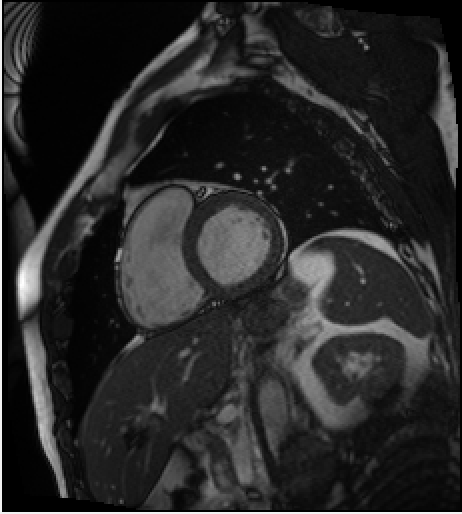
\includegraphics[width=200]{before.png}
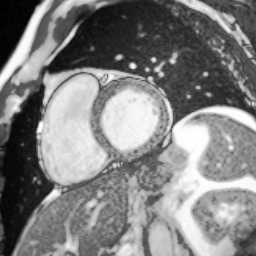
\includegraphics[width=200]{after.png}
\end{center}

Cele dou\u{a} imagini de mai sus reprezint\u{a} un exempu de imagine din setul de date \^{i}nainte de a fi procesat\u{a} \c{s}i dup\u{a} ce a fost procesat\u{a}, cum se poate observa imaginea procesat\u{a} a fost decupat\u{a} din mijlocul imaginii neprocesate, astfel \^{i}nc\^{a}t s\u{a} se elimine o cantitate c\^{a}t mai mare de date care nu sunt necesare pentru scopul nostru, de asemenea se mai poate observa c\u{a} imaginea procesat\u{a} are un contrast mai mare fa\c{t}\u{a} de imaginea neprocesat\u{a}, iar detaliile imaginii se pot observa mai bine, aceste lucruri vor duce la o vitez\u{a} de calcul \c{s}i la o acurate\c{t}e mai mare a re\c{t}elei neuronale.

\par

Cum am precizat mai sus, vom salva intr-un fi\c{s}ier CSV id-ul pacientului, numarul radiografiei, numarul imaginii, numarul de linii \c{s}i de coloane, distan\c{t}a fizic\u{a} \^{i}ntre centrii a doi pixeli, ad\^{a}ncimea radiografiei, locatia radiografiei, planul in care a fost facut\u{a} radiografia ( pe line sau pe coloan\u{a} ) \c{s}i pozi\c{t}ia imaginii fa\c{t}\u{a} de col\c{t}ul din st\^{a}nga sus, pe l\^{a}ng\u{a} toate acestea vom mai salva \c{s}i varianta prin care s-a facut radiografia, c\^{a}nd s-a f\u{a}cut radiografia, firma care a f\u{a}cut aparatul de RMN \c{s}i numele modelului, v\^{a}rsta pacientului, ziua de na\c{s}tere a pacientului, sexul pacientului, numele fi\c{s}ierului \c{s}i orientarea pacientului in imagine. DICOM define\c{s}te un sistem de coordonate numit RCS (Reference Coordinates System) prin care se stabile\c{s}te pozi\c{t}ia corpului  \^{i}n imagine, astfel c\u{a} direc\c{t}ia X este de la m\^{a}na dreapta a pacientului spre m\^{a}na st\^{a}ng\u{a} a acestuia, direc\c{t}ia Y este din fa\c{t}a pacientului spre spatele acestuia, iar direc\c{t}ia Z este de la picioare spre cap, din cauza faptului c\u{a} pozi\c{t}ia corpului este tridimensional\u{a}, iar radiografia este bidimensional\u{a} se va calcula proiec\c{t}ia fiecarei axe definite mai sus la axele unui plan bidimensional, \^{i}n acest caz \^{i}n formatul DICOM se vor gasi \c{s}ase valori care definesc orientarea pacientului in imagine. Primele trei valori reprezint\u{a} proiec\c{t}ia celor trei axe a planului tridimensional la axa X a planului bidimensional (Xx, Xy, Xz), iar celelalte trei valori reprezint\u{a} proiec\c{t}ia celor trei axe a planului tridimensional la axa Y a planului bidimensional (Yx, Yy, Yz), cu aceste valori se poate stabilii foarte u\c{s}or cum este orientat un pacient intr-o radiografie.

\par

Toate valorile salvate mai sus \^{i}n fi\c{s}ierul CSV au fost valori pe care nu am fost nevoi\c{t}i s\u{a} le calcul\u{a}m doarece sunt deja existente \^{i}n fiecare radiografie, \^{i}ns\u{a} pe baza lor putem s\u{a} calcul\u{a}m noi valori care ne vor fi de folos pe parcurs. Una dintre acestea este s\u{a} stabilim timpul dintre dou\u{a} imagini consecutive dintr-o radiografie \c{s}i distan\c{t}a dintre loca\c{t}iile lor, acestea pot fi u\c{s}or calculate prin diferen\c{t}a dintre timpii  celor dou\u{a} imagini \c{s}i a pozi\c{t}iilor pe care le au.

\section{Identificarea ventriculului st\^{a}ng}

Cum se poate observa \c{s}i \^{i}n imaginea de mai jos ventriculul st\^{a}ng este destul de u\c{s}or de identificat cu ochiul liber pentru un om, \^{i}ns\u{a} pentru un calculator aceasta este \^{i}nc\u{a} greu de g\u{a}sit.

\par

Pentru a putea identifica ventriculul st\^{a}ng din astfel de imagine vom avea nevoie de o re\c{t}ea neuronal\u{a} care s\u{a} fac\u{a} segmentarea ventriculului st\^{a}ng de restul de date, iar dup\u{a} aceea se va putea folosii rezultatul ob\c{t}inut pentru calcularea volumului de s\^{a}nge care curge la sistol\u{a} \c{s}i a volumului de s\^{a}nge care curge la diastol\u{a}.

\par

Pentru antrenarea re\c{t}elei neuronale care va face segmentarea inimii vom avea nevoie de un alt set de date, deoarece setul de date pe care \^{i}l avem de la Institutul Na\c{t}ional pentru Inim\u{a}, Pl\u{a}m\^{a}ni \c{s}i S\^{a}nge din America nu ne ofer\u{a} date care s\u{a} indice pozi\c{t}ia exact\u{a} a ventriculului st\^{a}ng \^{i}n radiografie, \^{i}ns\u{a} spitalul Sunnybrook din Canada, Toronto pune la dispozi\c{t}ie date identice care ne ofer\u{a} pozi\c{t}ia exact\u{a} a ventriculului st\^{a}ng \^{i}n radiografie.

\begin{center}
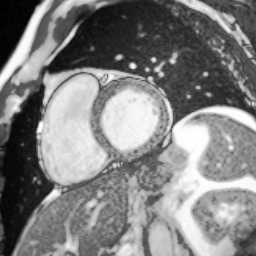
\includegraphics[width=200]{after.png}
\end{center}

\subsection{Datele de la spitalul Sunnybrook}

Cum am precizat \c{s}i mai sus, spitalul Sunnybrook pune la dispozi\c{t}ie un set de date care arat\u{a} pozi\c{t}ia exact\u{a} a ventricului st\^{a}ng a inimii \^{i}n radiografie. Fiecare radiografie a fost f\u{a}cut\u{a} pe parcursul a unui ciclu a inimii, av\^{a}nd o dimensiune de [ 256 x 256 ] de pixeli, iar pentru fiecare radiografie este asociat  un fisier txt cu pozi\c{t}ia exact\u{a} a ventricului st\^{a}ng a inimii.

\begin{center}
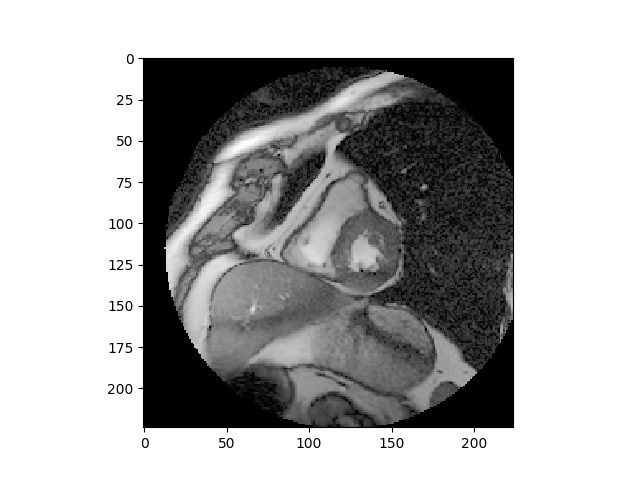
\includegraphics[width=200]{sbh.png}
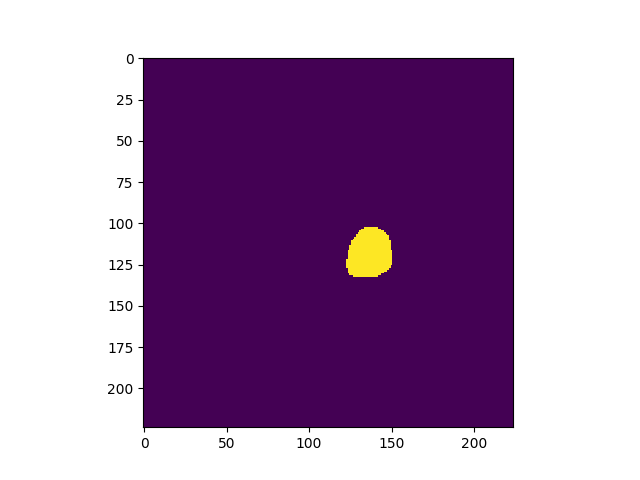
\includegraphics[width=200]{sbl.png}
\end{center}

\^{I}n imaginile de mai sus, avem o radiografie din setul de date Sunnybrook \^{i}n partea din st\^{a}nga, iar \^{i}n partea din dreapta avem pozi\c{t}ia exact\u{a} a ventricului st\^{a}ng \^{i}n radiografie, unde ce este colorat cu mov reprezint\u{a} faptul c\u{a} acolo nu se afl\u{a} ventriculul st\^{a}ng (culoarea mov are asociat\u{a} valoarea 0), iar ce este colorat cu galben reprezint\u{a} faptul c\u{a} acolo se afl\u{a} ventriculul st\^{a}ng (culoarea galben\u{a} are asociat\u{a} valoarea 1). Cu astfel de tipuri de date vom lucra pentru a antrena o re\c{t}ea neuronal\u{a} care s\u{a} fac\u{a} segmentarea ventricului st\^{a}ng a inimii de restul radiografiei. 

\par

La final dup\u{a} ce vom termina s\u{a} antren\u{a}m re\c{t}eaua neuronal\u{a}, vom introduce radiografii de la Institutul Na\c{t}ional pentru Inim\u{a}, Pl\u{a}m\^{a}ni \c{s}i S\^{a}nge din America, ca radiografia de mai sus din st\^{a}nga, iar la final vom ob\c{t}ine pozi\c{t}ia exact\u{a} a ventricului st\^{a}ng, ca \^{i}n imaginea din dreapta, unde 0 reprezint\u{a} faptul c\u{a} pixelul de la pozi\c{t}ia respectiv\u{a} nu apar\c{t}ine ventricului st\^{a}ng, iar valoarea 1 reprezint\u{a} faptul c\u{a} pixelul de la pozi\c{t}ia respectiv\u{a} apar\c{t}ine ventricului st\^{a}ng, iar pe baza acestor valori vom putea face segmentarea.

\subsection{Preprocesarea setului de date Sunnybrook}

Primul pas pe care trebuie s\u{a} \^{i}l facem \^{i}nainte de a introduce setul de date Sunnybrook \^{i}ntr-o re\c{t}ea neuronal\u{a} este de al preprocesa. La fel cum am facut \c{s}i mai sus, vom citi fiecare fi\c{s}ier DICOM, vom extrage din el doar radiografia, vom aplica metoda CLAHE pentru a \^{i}mbun\u{a}t\u{a}\c{t}ii contrastul \c{s}i calitatea radiografiei iar la final vom salva rezultatul ob\c{t}inut \^{i}ntr-un fi\c{s}ier PNG pentru a fi mai u\c{s}or de citit \c{s}i de vizualizat.

\subsection{Re\c{t}ele neuronale pentru segmentarea ventricului st\^{a}ng}

Arhitectura re\c{t}elei neuronale pe care am aleso, pentru segmentarea ventricului st\^{a}ng de restul radiografiei, a fost inspirat\u{a} din arhitectura re\c{t}elei neuronale pe care cei de la Universatea Oxford au construito pentru a segmenta categorii de obiecte dintr-o imagine, dar din cauza faptului c\u{a} modelul celor de la Oxford, numit Visual Geometry Group ( prescurtat VGG ), dup\u{a} grupul care a venit cu idee acestei arhitecturi, era foarte complex\u{a} \c{s}i se ajungea u\c{s}or la efectul de overfitting, acesta a trebuit simplificat\u{a,} astfle \^{i}nc\^{a}t s\u{a} se evite pe c\^{a}t posibil efectul de overfitting.

\par

Dup\u{a} \^{i}ncercarea multor varia\c{t}ii a arhitecutrii VGG, prin care am \^{i}ncercat s\u{a} atingem un scor la func\c{t}ia de cost c\^{a}t mai mic \c{s}i prin care s\u{a} avem o precizie la datele de test c\^{a}t mai bun\u{a}, am ajuns la urm\u{a}toarea arhitectur\u{a} pentru segmentorul nostru.

\begin{center}
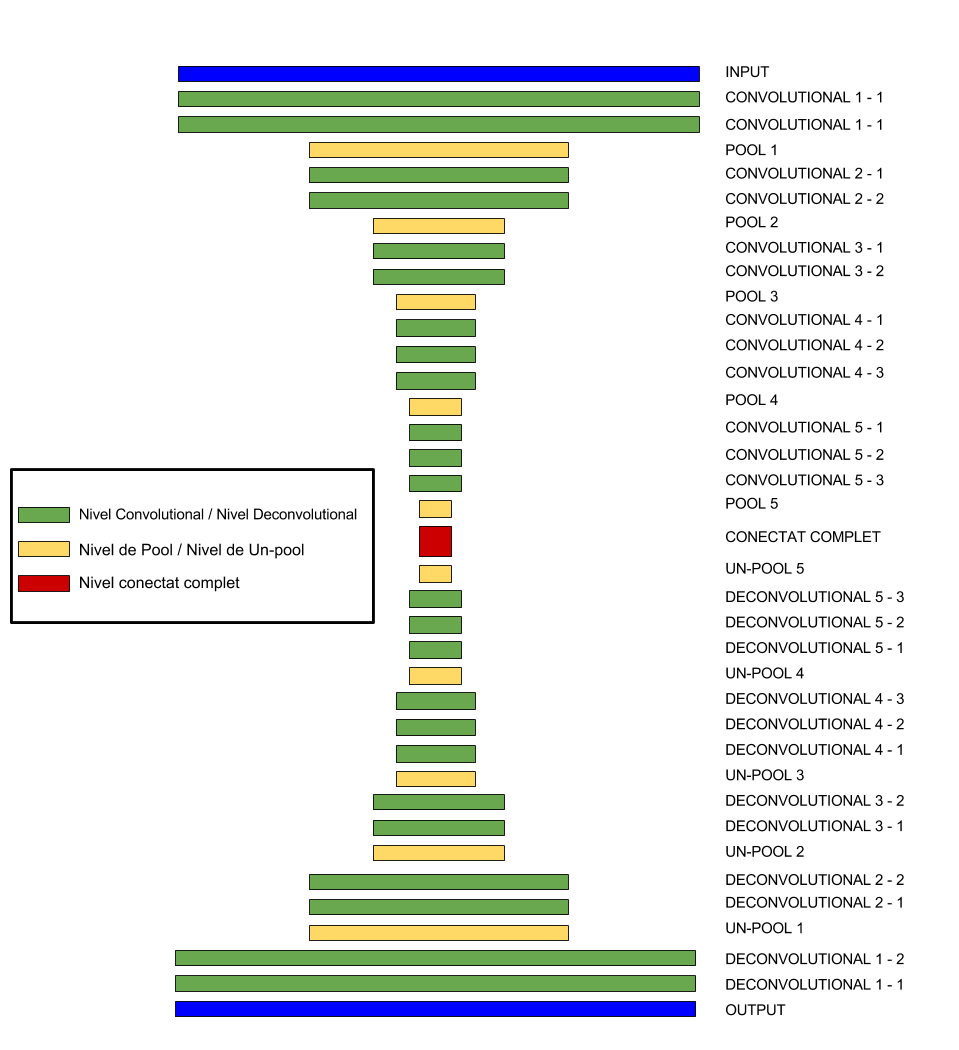
\includegraphics[width=500]{arhitectura_segmentor.png}
\end{center}

\^{I}n imaginea de mai sus am ilustrat nivelele din re\c{t}eaua neuronal\u{a}, unde am reprezentat prin culoarea verde nivelele convolu\c{t}ionale \c{s}i deconvolu\c{t}ionale, prin galben nivelele de pool \c{s}i de un-pool, iar prin ro\c{s}u nivelul conectat complet.

\par

Nivelele deconvolu\c{t}ionale \c{s}i nevelele de un-pool sunt nivele ce se comport\u{a} invers fa\c{t}\u{a} de nivelul convolu\c{t}ionl, respectiv nivelul de pool. Mai exact, nivelul de un-pool m\u{a}re\c{s}te spa\c{t}iul dimensional pe baza pozi\c{t}iilor care au trecut de nivelul de pool, iar nivelul deconvolu\c{t}ional este de fapt transpusa nivelului convolu\c{t}ional.

\par

\^{I}n arhitectura ilustrat\u{a} mai sus, am pus dup\u{a} fiecare nivel convolu\c{t}ional c\^{a}te o func\c{t}ie de activare ReLU, iar nivelele convolu\c{t}ionale \c{s}i deconvolu\c{t}ionale au ponderi de dimensiune [3x3] cu un pas de glisare a ferestrei egal cu unu \^{i}n toate direc\c{t}iile de deplasere. Am ini\c{t}ializat ponderile de la nivelele convolu\c{t}ionale \c{s}i deconvolu\c{t}ionale cu variabile aleatoare dintr-o distribu\c{t}ie normal\u{a}, unde devia\c{t}ia standard este setat\u{a} la $\frac{1}{\sqrt{n}}$, unde n reprezint\u{a} numarul de variabile, iar bias-ul a fost setat la valoarea zero. Padding-ul a fost setat astfel \^{i}nc\^{a}t dimensiunea datelor de intrare, pe lungime \c{s}i \^{i}n\u{a}l\c{t}ime, s\u{a} se p\u{a}streze la datele rezultate \^{i}n urma aplic\u{a}rii nivelelor convolu\c{t}ionale \c{s}i deconvolu\c{t}ionale.

\par

Nivelul de pool \c{s}i un-pool, le-au fost setate o fereastr\u{a} de dimensiune [2x2] cu un pas de glisare a ferestrei egal cu doi, astfle \^{i}nc\^{a}t cantitatea de date s\u{a} se reduc\u{a} cu un procent de 75\% dup\u{a} aplicarea unui nivel de pool, respectiv s\u{a} se mareasc\u{a} cu un procent de 75\% dup\u{a} aplicarea unui nivel de un-pool.

\begin{center}
 \begin{longtable}{|p{4cm}|p{3cm}|p{3cm}|p{3cm}|} 
 \hline
 Nume & Dimensiune date de intrare & Numar ponderi \c{s}i bias-uri & Dimensiune date de ie\c{s}ire \\ [0.5ex] 
 \hline\hline
 Convolutional 1 - 1 &  [224 x 224 x 1] & 32 & [224 x 224 x 32] \\ 
 \hline
 Convolutional 1 - 2 & [224 x 224 x 32] & 32 & [224 x 224 x 32] \\
 \hline
 Pool 1 & [224 x 224 x 32] & - & [112 x 112 x 32] \\
 \hline
 Convolutional 2 - 1 & [112 x 112 x 32] & 64 & [112 x 112 x 64] \\
 \hline
 Convolutional 2 - 2 & [112 x 112 x 64] & 64 & [112 x 112 x 64] \\
 \hline
 Pool 2 & [112 x 112 x 64] & - & [56 x 56 x 64] \\
 \hline
 Convolutional 3 - 1 & [56 x 56 x 64] & 128 & [56 x 56 x 128] \\
 \hline
 Convolutional 3 - 2 & [56 x 56 x 128] & 128 & [56 x 56 x 128] \\
 \hline
 Pool 3 & [56 x 56 x 128] & - & [28 x 28 x 128] \\
 \hline
 Convolutional 4 - 1 & [28 x 28 x 128] & 256 & [28 x 28 x 256] \\
 \hline
 Convolutional 4 - 2 & [28 x 28 x 256] & 256 & [28 x 28 x 256] \\
 \hline
 Convolutional 4 - 3 & [28 x 28 x 256] & 256 & [28 x 28 x 256] \\
 \hline
 Pool 4 & [28 x 28 x 256] & - & [14 x 14 x 256] \\
 \hline
 Convolutional 5 - 1 & [14 x 14 x 256] & 256 & [14 x 14 x 256] \\
 \hline
 Convolutional 5 - 2 & [14 x 14 x 256] & 256 & [14 x 14 x 256] \\
 \hline
 Convolutional 5 - 3 & [14 x 14 x 256] & 256 & [14 x 14 x 256] \\
 \hline
 Pool 5 & [7 x 7 x 256] & - & [7 x 7 x 256] \\
 \hline
 Conectat complet & [7 x 7 x 256] & 4096 & [1 x 1 x 4096] \\
 \hline
 Deconectat complet & [1 x 1 x 4096] & 256 & [7 x 7 x 256] \\
 \hline
 Un-pool 5  & [7 x 7 x 256] & - & [14 x 14 x 256] \\
 \hline
 Deconvolutional 5 - 3 & [14 x 14 x 256] & 256 & [14 x 14 x 256] \\
 \hline
 Deconvolutional 5 - 2 & [14 x 14 x 256] & 256 & [14 x 14 x 256] \\
 \hline
 Deconvolutional 5 - 1 & [14 x 14 x 256] & 256 & [14 x 14 x 256] \\
 \hline
 Un-pool 4  & [14 x 14 x 256] & - & [28 x 28 x 256] \\
 \hline
 Deconvolutional 4 - 3 & [28 x 28 x 256] & 256 & [28 x 28 x 256] \\
 \hline
 Deconvolutional 4 - 2 & [28 x 28 x 256] & 256 & [28 x 28 x 256] \\
 \hline
 Deconvolutional 4 - 1 & [28 x 28 x 256] & 128 & [28 x 28 x 128] \\
 \hline
 Un-pool 3  & [28 x 28 x 128] & - & [56 x 56 x 128] \\
 \hline
 Deconvolutional 3 - 2 & [56 x 56 x 128] & 128 & [56 x 56 x 128] \\
 \hline
 Deconvolutional 4 - 1 & [56 x 56 x 128] & 64 & [56 x 56 x 64] \\
 \hline
 Un-pool 2  & [56 x 56 x 64] & - & [112 x 112 x 64] \\
 \hline
 Deconvolutional 2 - 2 & [112 x 112 x 64] & 64 & [112 x 112 x 64] \\
 \hline
 Deconvolutional 2 - 1 & [112 x 112 x 64] & 32 & [112 x 112 x 32] \\
 \hline
  Un-pool 1  & [112 x 112 x 32] & - & [224 x 224 x 32] \\
 \hline
 Deconvolutional 1 - 2 & [224 x 224 x 32] & 32 & [224 x 224 x 32] \\
 \hline
 Deconvolutional 1 - 1 & [224 x 224 x 32] & 32 & [224 x 224 x 32] \\
 \hline
 Output & [224 x 224 x 32] & 2 & [224 x 224 x 2] \\
 \hline
 Softmax & [224 x 224 x 2] & - & [224 x 224 x 2] \\
 \hline
 Argmax & [224 x 224 x 2] & - & [224 x 224 x 1] \\
 \hline
\end{longtable}
\end{center}

Cum am precizat \c{s}i mai sus, nivelele convolu\c{t}ionale \c{s}i deconvolu\c{t}ionale au ponderi de dimensiune [3 x 3], singurile nivele care nu respect\u{a} acest\u{a} dimensiune, sunt nivelele Conectat complet \c{s}i Deconectat complet, unde ponderile au o dimensiune de [7 x 7] pentru a conecta fiecare neuron cu fiecare ponder\u{a}. Alt nivel care nu respect\u{a} aceast\u{a} dimensiune este nivelul de Output, care are o dimensiune a ponderilor de [1 x 1], acest nivel are rolul de a aduce dimensiunea datelor, de la penultimul nivel deconvolu\c{t}ional, de la valoarea 32 la numarul de clase posbile, \^{i}n cazul nostru sunt doua clase posibile, exist\u{a} sau nu la pozi\c{t}ia respectiv\u{a} ventirculul st\^{a}ng a inimii, aceste clase sunt reprezentate prin valoarea 1 pentru posibilitatea c\u{a} exist\u{a} \c{s}i 0 pentru posibilitatea c\u{a} nu exist\u{a}.

\par

Dup\u{a} nivelul de Output se aplic\u{a} func\c{t}ia Softmax, ca func\c{t}ie de cost, pentru calcularea pierderii, iar pentru aflarea rezultatului final se aplic\u{a} o func\c{t}ie numit\u{a} Argmax, care \^{i}ntoarce pozi\c{t}ia unde valoarea este cea mai mare, aceast\u{a} func\c{t}ie este aplicat\u{a} pe ad\^{a}ncimea setului de date. Ceea ce \^{i}ntoarce func\c{t}ia Argmax reprezint\u{a} prezicerile pe care re\c{t}eaua neuronal\u{a} o face \^{i}n urma procesului de antrenare.

\par

\^{I}nainte ca setul de date de la spitalul Sunnybrook s\u{a} fie introduce \^{i}n re\c{t}eaua neuronal\u{a}, \^{i}n procesul de antrenare sau pentru preziceri, acestea trebuiesc mai \^{i}nt\^{a}i decupate astfel \^{i}nc\^{a}t s\u{a} intre \^{i}n re\c{t}eaua neuronal\u{a}. Cum se observ\u{a} \c{s}i \^{i}n tabelul de mai sus, re\c{t}eaua neuronal\u{a} accept\u{a} un set de date de dimensiunea [224 x 224], \^{i}ns\u{a} setul de date de la Sunnybrook are o dimensiune de [254 x 256]. Acest lucur a fost f\u{a}cut pentru a multimplica setul de date, din cauz\u{a} c\u{a} setul de date pus la dispozi\c{t}ie de spitalul Sunnybrook este destul de mic ( doar 805 de exemple ), trebuia s\u{a} gasim o modalitate de al multiplica, iar cea mai bun\u{a} solu\c{t}ie pe care am gasito pentru a face acest lucru a fost s\u{a} punem re\c{t}eaua neuronal\u{a} s\u{a} accepte un volum de date de dimensiune mai mic\u{a}, astfel \^{i}nc\^{a}t s\u{a} putem sa decup\u{a}m la o pozi\c{t}ie aleatoare setul de date. Prin urmare, \^{i}nainte s\u{a} introducem setul de date \^{i}n re\c{t}eaua neuronal\u{a}, alegem dou\u{a} valori aleatorii, una pentru axa Ox, alta pentru axa Oy, \c{s}i incepem s\u{a} decup\u{a}m de la acea pozi\c{t}ie, dup\u{a} aceea setul de date  decupat este centrat la zero \c{s}i normalizat, setul de date rezultat este introdus \^{i}n re\c{t}eaua neuronalu\u{a}.

\par

La procesul de antrenare,  am ales metoda Adam pentru antrenare, rata de \^{i}nv\u{a}\c{t}are a fost setat\u{a} la valoarea de 1e-6, \c{s}i s-au efectuat 40 de itera\c{t}ii peste setul de date, iar la fiecare pas de antrenare s-au luat c\^{a}te doua exemple din setul de date. Din cele 805 de exemple de antrenare, puse la dispozi\c{t}ie de spitalul Sunnybrook, am p\u{a}strat 5 valori pentru a vedea ce preziceri face re\c{t}eaua neuronal\u{a} peste date pe care nu le-a vazut niciodat\u{a} \^{i}n procesul de antrenare, celelate 800 de exemple au fost folosite \^{i}n procesul de antrenare. Cu 800 de exemple de antrenare, din care s-au luat 2 exemple la fiecare pas de antrenare, la fiecare pas de itera\c{t}ie peste setul de date s-au efectuat 400 de pa\c{s}i de antrenare, av\^{a}nd \^{i}n vedere c\u{a} s-au f\u{a}cut 40 de itera\c{t}ii peste setul de dat avem un total de 160.000 de pa\c{s}i de antrenare. L-a fiecare itera\c{t}ie peste setul de date ( numit si epoch ) s-au salvat parametrii re\c{t}elei neuronale \c{s}i s-a calculat func\c{t}ia total\u{a} de cost peste setul de date.

\begin{center}
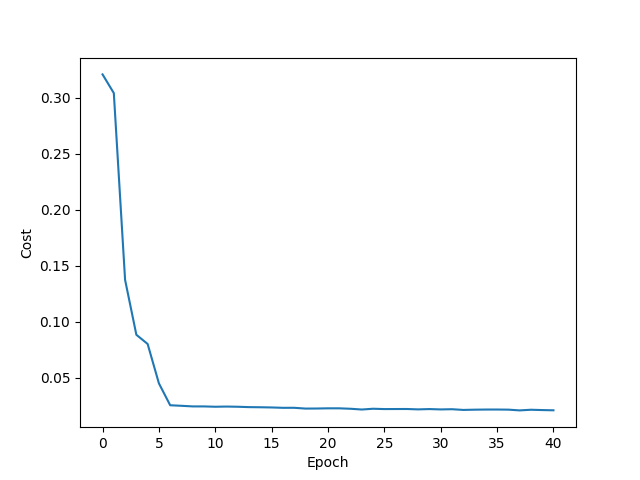
\includegraphics[width=400]{loss.png}
\end{center}

\^{I}n graficul de mai sus s-a ilustrat progresul func\c{t}iei de cost la fiecare epoch, ce-a mai mic\u{a} valoare a fost atins\u{a} la epoch-ul 40, unde func\c{t}ia de cost a ar\u{a}tat o valoare de 0.019257. Procesul de antrenare a durat 5 ore pe un nvidia geforce titan x, iar re\c{t}eaua neuronal\u{a} a fost scris\u{a} in Python 3.5 cu ajutorul libr\u{a}riei TensorFlow.

\^{I}n imaginile de mai jos pute\c{t}i vedea prezicerile pe care re\c{t}eaua neuronal\u{a} le-a f\u{a}cut pe seteul de date care nu a fost inclus \^{i}n procesul de antrenare ( cele 5 exemple ). Motivul pentru care se exclud unele date din procesul de antrenare pentru a se face preziceri pe ele este acela de a vedea cum se descurc\u{a} re\c{t}eaua neuronal\u{a} pe un set de date pe care nu l-a vazut niciodat\u{a} \c{s}i pentru a ne asigura c\u{a} re\c{t}eaua neuronal\u{a} nu a \^{i}nv\u{a}\c{t}at pe dinafar\u{a} datele de antrenare ( efectul de overfitting ).

\par

Setul de imagine pe care le vom prezenta, \^{i}n cele ce urmeaz\u{a}, sunt structurate pe dou\u{a} coloane, pe prima coloan\u{a} sunt raspunsurile, pe care re\c{t}eaua neuronal\u{a} ar trebuii s\u{a} le prezic\u{a}, iar pe a do\u{a} coloan\u{a} sunt prezicerile pe care le-a facut re\c{t}eaua neuronal\u{a}. Pe fiecare coloana exist\u{a} trei randuri de imagini, unde pe primul r\^{a}nd este imagine pe care se face prezicerea, pe al doilea r\^{a}nd este prezicerea f\u{a}cut\u{a}, iar pe r\^{a}ndul trei este imaginea decupat\u{a} de pe primul r\^{a}nd pe baza prezicerilor de pe r\^{a}ndul doi.

\begin{center}
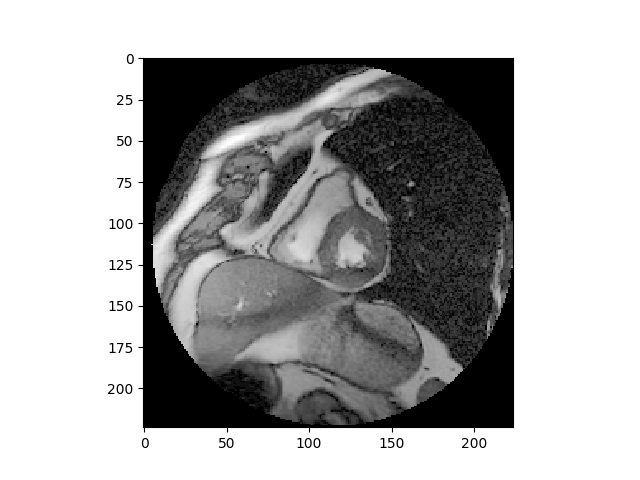
\includegraphics[width=200]{1_image.png}
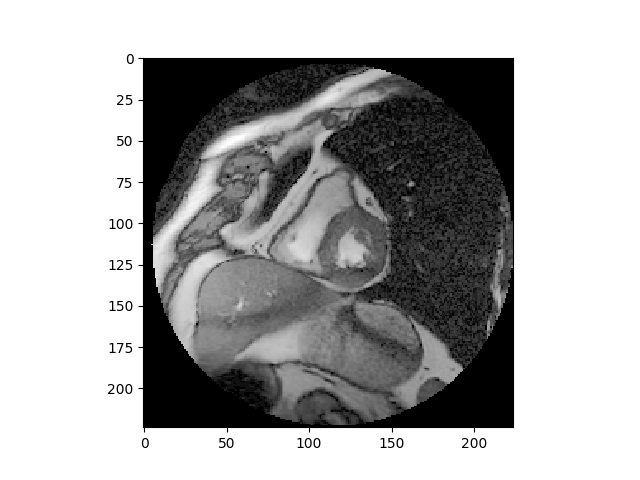
\includegraphics[width=200]{1_image.png}
\end{center}

\begin{center}
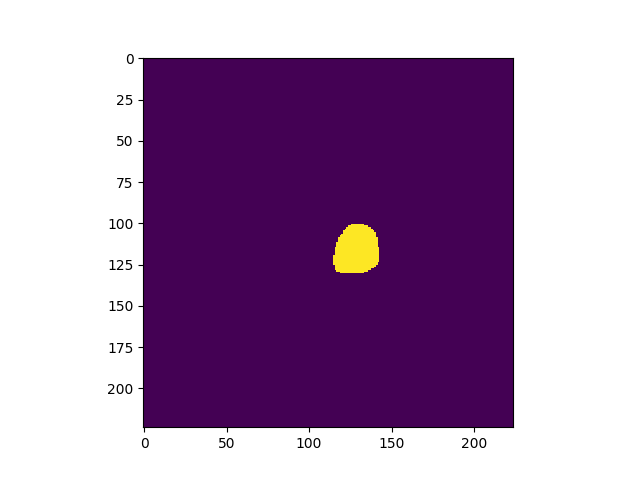
\includegraphics[width=200]{1_labels.png}
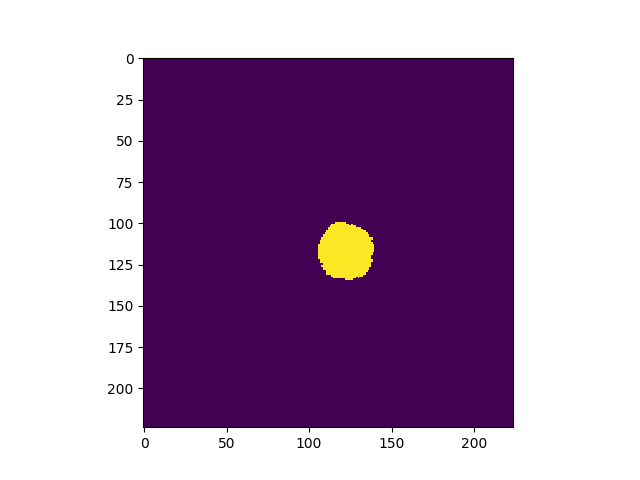
\includegraphics[width=200]{1_labels_predict.png}
\end{center}

\begin{center}
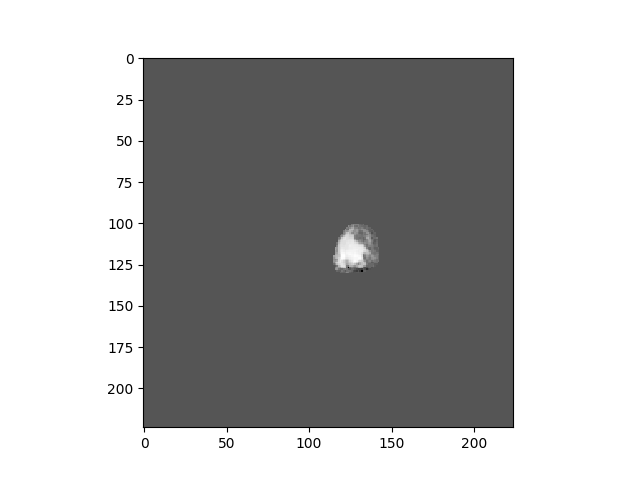
\includegraphics[width=200]{1_image_labels.png}
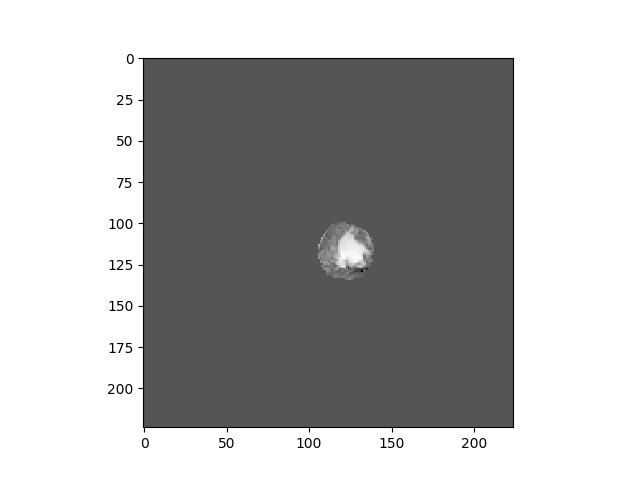
\includegraphics[width=200]{1_image_predict.png}
\end{center}

\^{I}n imaginile de mai sus, pe partea dtreapt\u{a}, sunt ilustrate rezultatele ob\c{t}inute la prezicere la primul exemplu, iar pe partea st\^{a}ng\u{a} este adev\u{a}rata valoare. Se poate observa faltul c\u{a}, prezicerea f\u{a}cut\u{a} de re\c{t}eaua neuronal\u{a} este destul de aproape de adev\u{a}r ( r\^{a}ndurile doi \c{s}i trei ), \^{i}ns\u{a} exist\u{a} diferen\c{t}e \^{i}ntre ele, cum ar fi spre exemplu faptul c\u{a} rec\c{t}eaua neuronal\u{a} a prezis ventriculul st\^{a}ng ceva mai la st\^{a}nga \c{s}i pu\c{t}in mai mare dec\^{a} era cu adev\u{a}rat.

\begin{center}
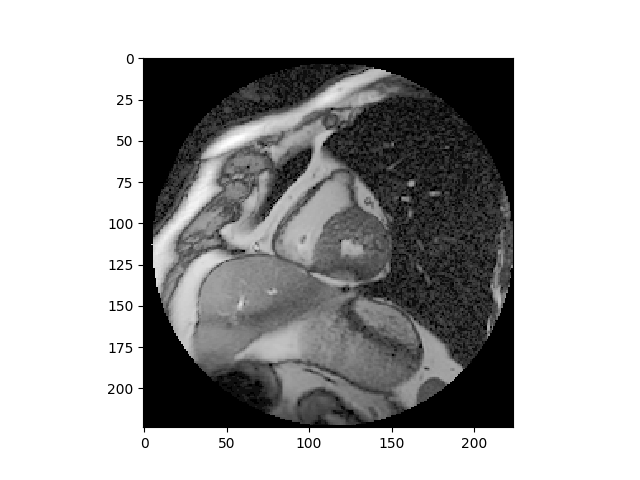
\includegraphics[width=200]{2_image.png}
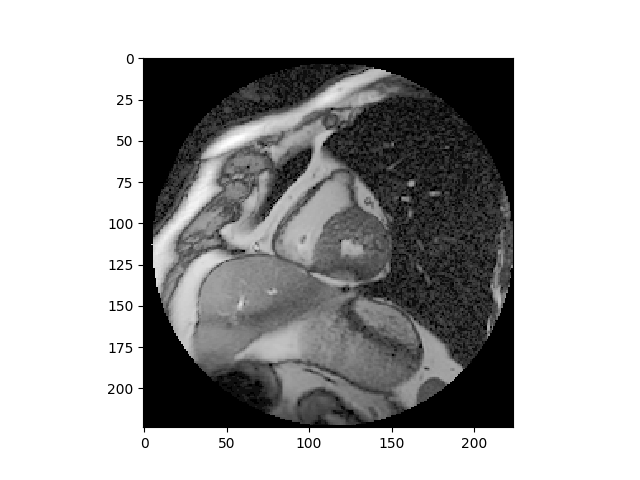
\includegraphics[width=200]{2_image.png}
\end{center}

\begin{center}
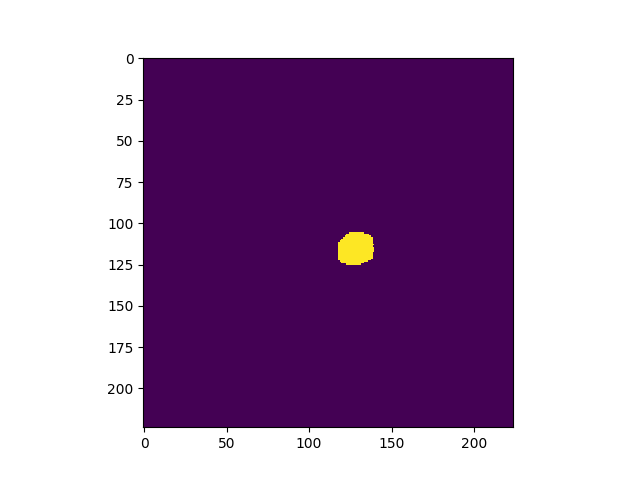
\includegraphics[width=200]{2_labels.png}
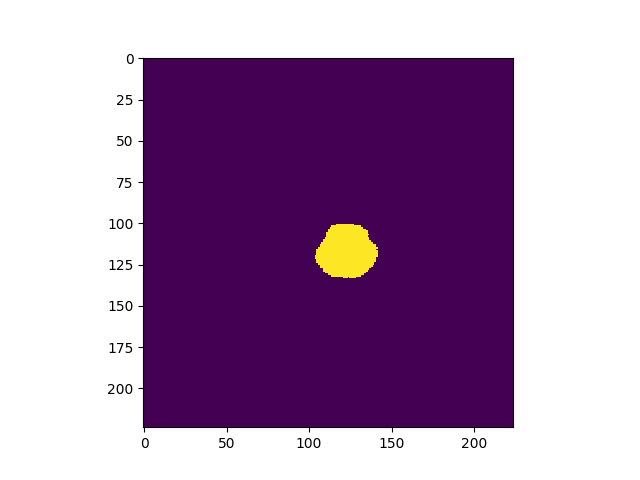
\includegraphics[width=200]{2_labels_predict.png}
\end{center}

\begin{center}
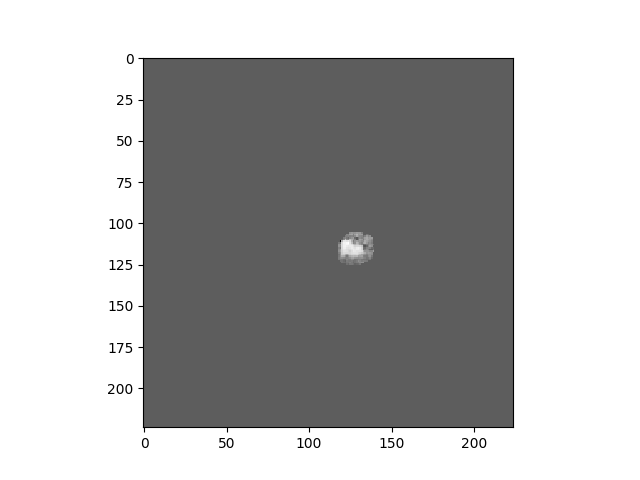
\includegraphics[width=200]{2_image_labels.png}
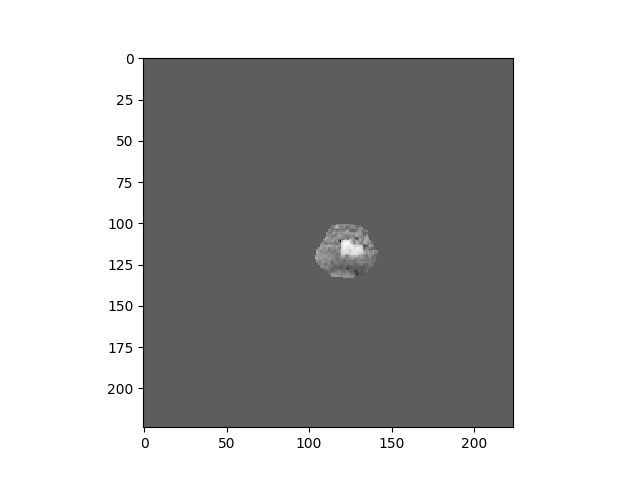
\includegraphics[width=200]{2_image_predict.png}
\end{center}

Prezicerea pe imaginea doi este ilustrat\u{a} mai sus. Se poate vedea c\u{a} rec\c{t}eaua neuronal\u{a} de data asta a prezis un ventricul st\^{a}ng mult mai mare de data asta dec\^{a}t era cu adev\u{a}rat. Acest lucru s-ar putea datora faptului c\u{a}, pe setul de imagini de antrenare, erau mai multe imagini cu ventriculul st\^{a}ng c\^{a}nd era la diastol\u{a} dec\^{a}t cele care erau la sistol\u{a}, iar din aceast\u{a} cauz\u{a} re\c{t}eaua neuronal\u{a} a prezis un ventricul st\^{a}ng a\c{s}a de mare, pentru c\u{a} a \^{i}nv\u{a}\c{t}at s\u{a} caute ventricule aflate la diastol\u{a}.

\begin{center}
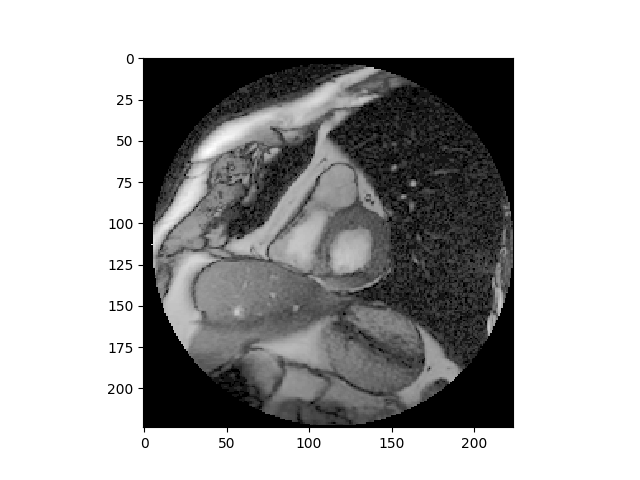
\includegraphics[width=200]{3_image.png}
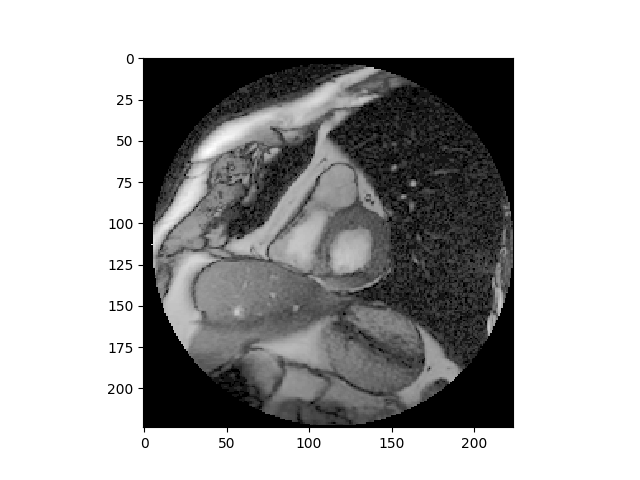
\includegraphics[width=200]{3_image.png}
\end{center}

\begin{center}
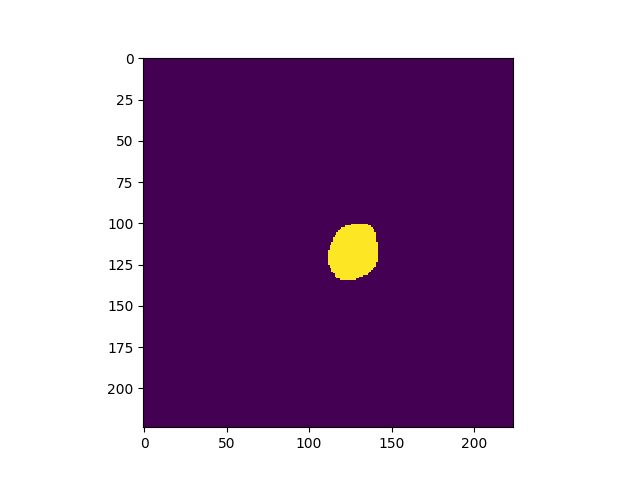
\includegraphics[width=200]{3_labels.png}
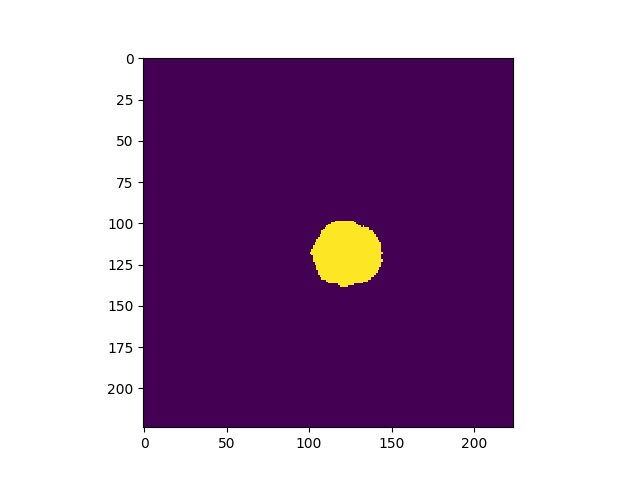
\includegraphics[width=200]{3_labels_predict.png}
\end{center}

\begin{center}
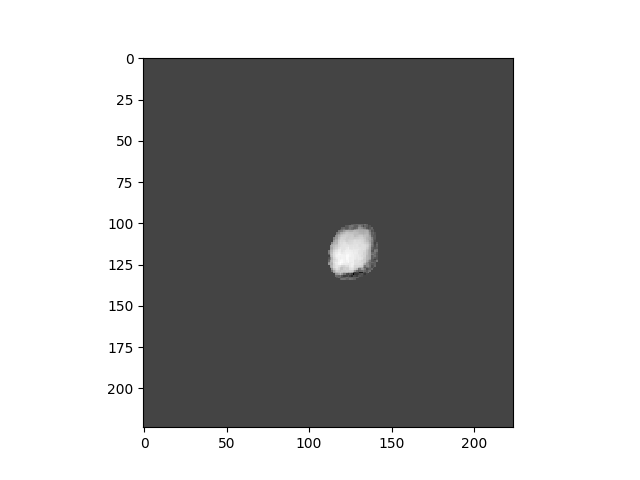
\includegraphics[width=200]{3_image_labels.png}
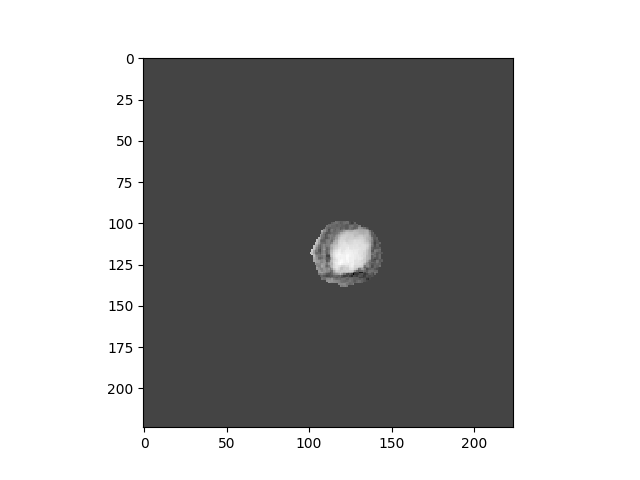
\includegraphics[width=200]{3_image_predict.png}
\end{center}

Pe setul de imagini trei, pe care s-a facut prezicerea de c\u{a}tre rec\c{t}eauan neuronal\u{a}, avem aceea\c{s}i problem\u{a}, re\c{t}eaua neuronal\u{a} face preziceri mult mari a ventricului st\^{a}ng dec\^{a}t sunt ele de fapt \^{i}n realitate. De data aceasta \^{i}ns\u{a} se poate trece cu vederea acest fapt, deoarece inima acum se afl\u{a} la diastol\u{a}, iar ventriculul st\^{a}ng este la expansiunea sa maxim\u{a}, iar prezicerea, dup\u{a} cum se poate observa, sunt destul de aproape de adev\u{a}r.

\begin{center}
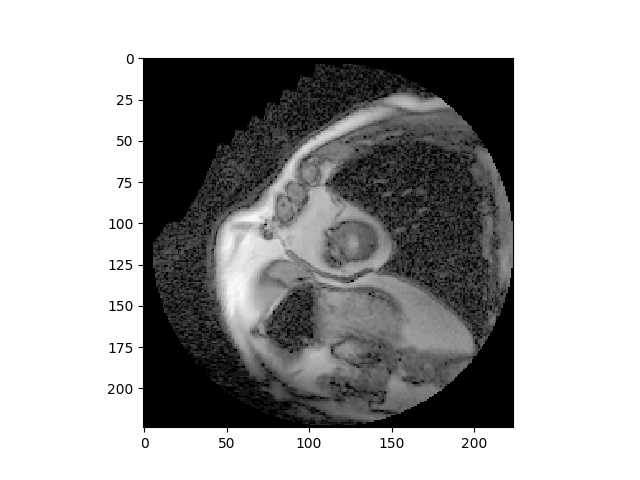
\includegraphics[width=200]{4_image.png}
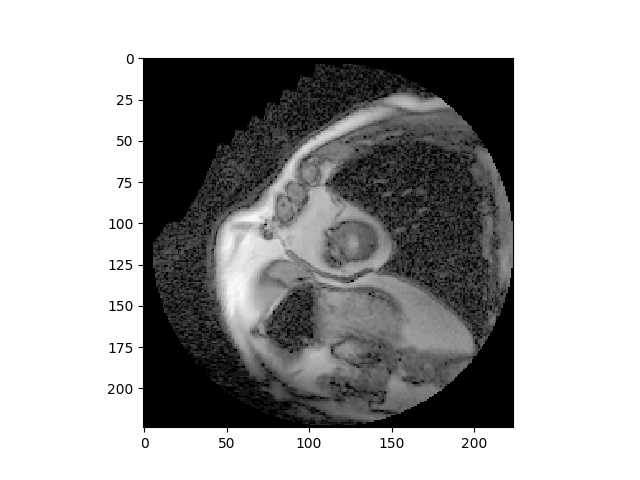
\includegraphics[width=200]{4_image.png}
\end{center}

\begin{center}
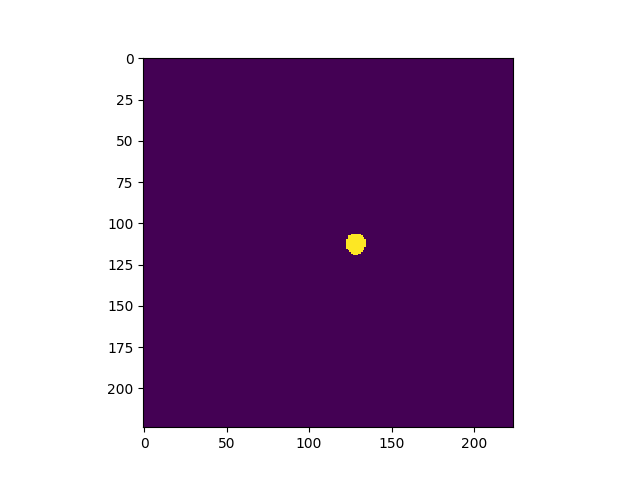
\includegraphics[width=200]{4_labels.png}
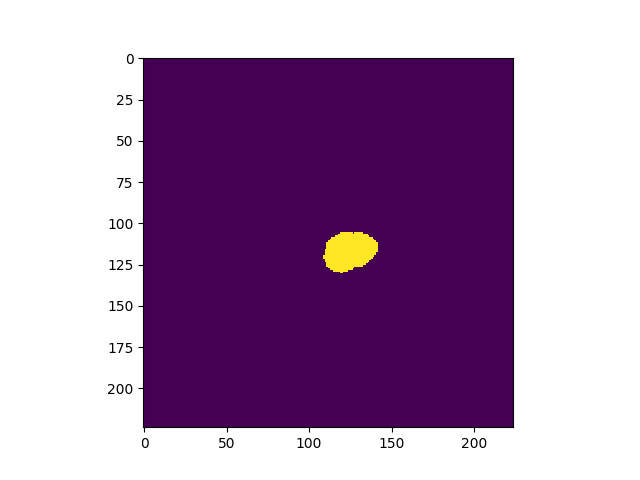
\includegraphics[width=200]{4_labels_predict.png}
\end{center}

\begin{center}
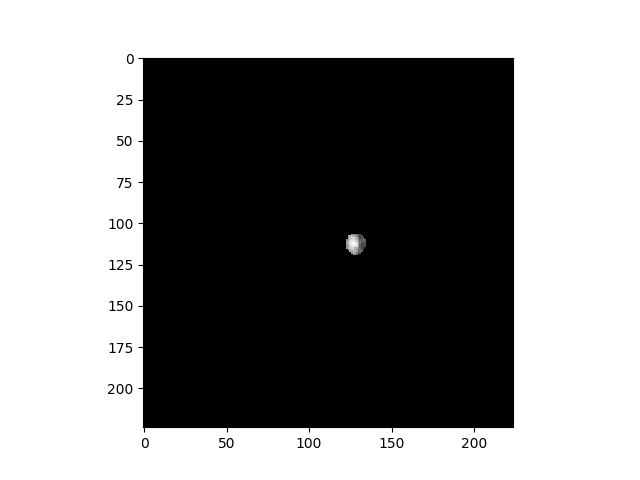
\includegraphics[width=200]{4_image_labels.png}
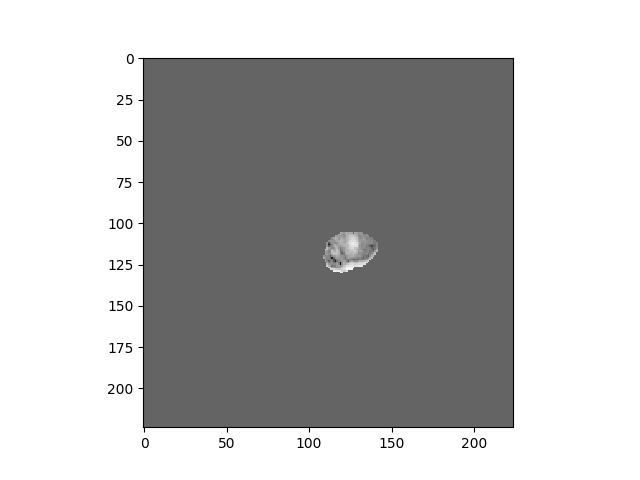
\includegraphics[width=200]{4_image_predict.png}
\end{center}

Penultimul set de date pe care s-a f\u{a}cut prezicerea este cel mai interesant, deoarece inima se afl\u{a} la sistol\u{a}, iar ventriculul st\^{a}ng este greu de detectat \c{s}i cu ochiul liber, \^{i}ns\u{a} re\c{t}eaua neuronal\u{a} a reu\c{s}it s\u{a} \^{i}l detecteze, ins\u{a} a facut iar aceea\c{s}i gre\c{s}teal\u{a} ca \c{s}i la celelalte cazuri, a dectectat un ventricul st\^{a}ng mult mai mare dec\^{a}t este el de fapt. Dup\u{a} cum se poate observa, ventriculul st\^{a}ng detectat acum de re\c{t}eaua neuronal\u{a} este de vreo cinci ori mai mare dec\^{a}t ar trebuii s\u{a} fie, acest lucru fiind pus pe seama faptului c\u{a}, \^{i}n setul de date de antrenare exist\u{a} pu\c{t}ine exeple cu un ventricul st\^{a}ng a\c{s}a de mic.

\begin{center}
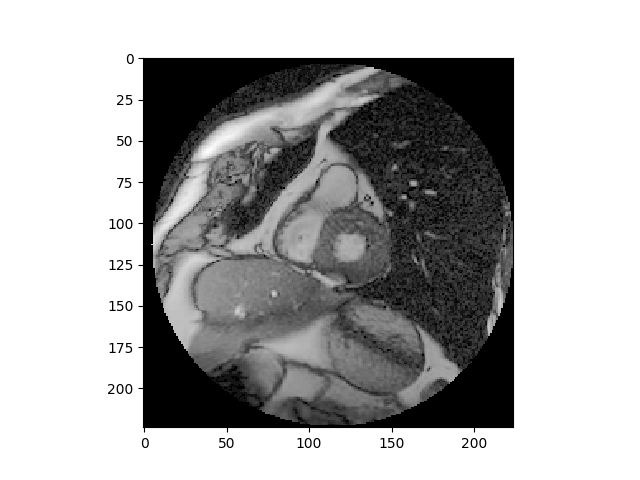
\includegraphics[width=200]{5_image.png}
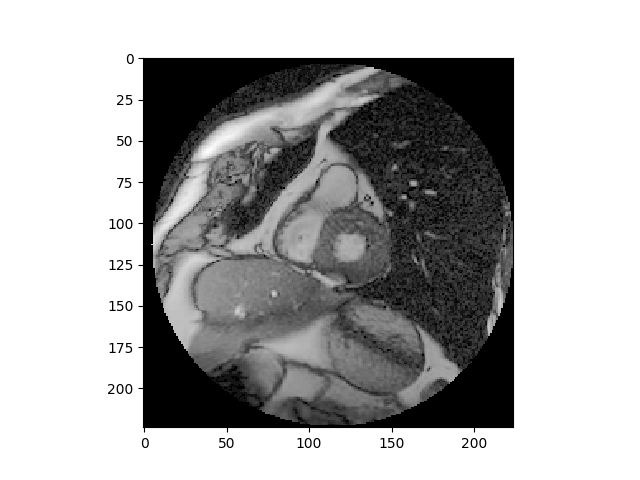
\includegraphics[width=200]{5_image.png}
\end{center}

\begin{center}
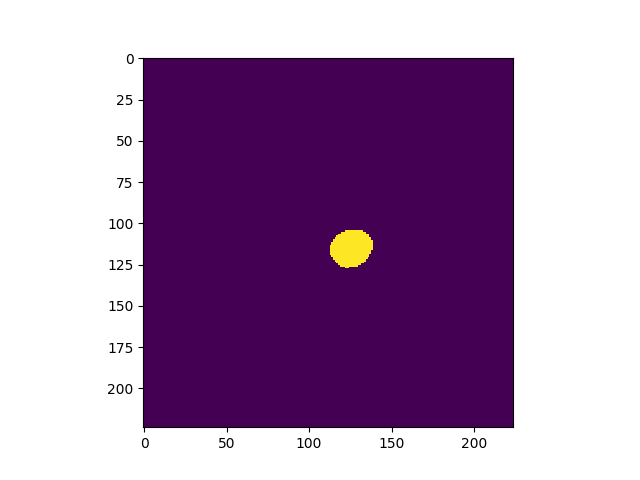
\includegraphics[width=200]{5_labels.png}
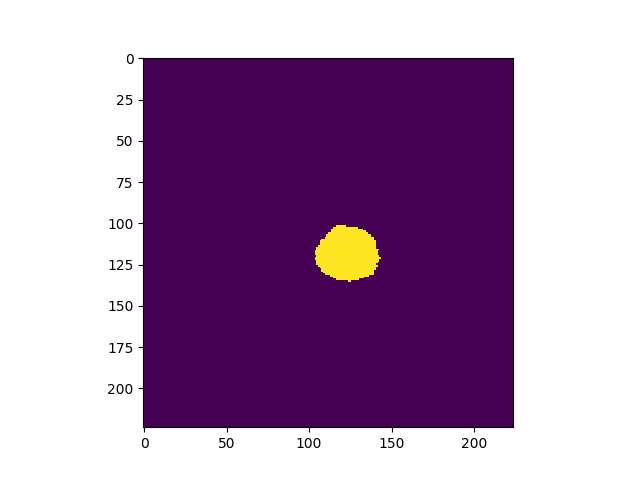
\includegraphics[width=200]{5_labels_true.png}
\end{center}

\begin{center}
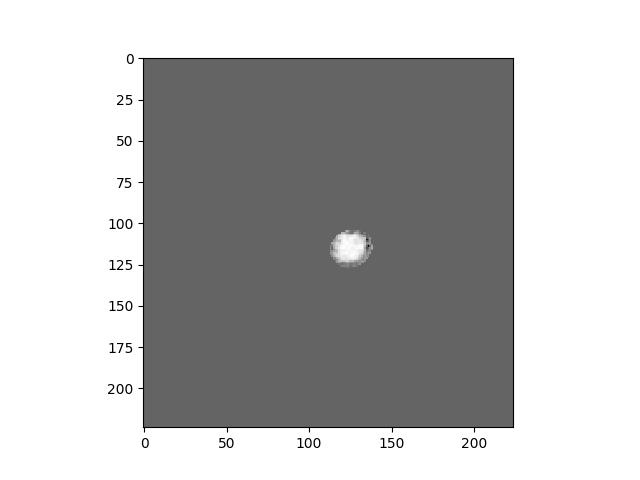
\includegraphics[width=200]{5_image_labels.png}
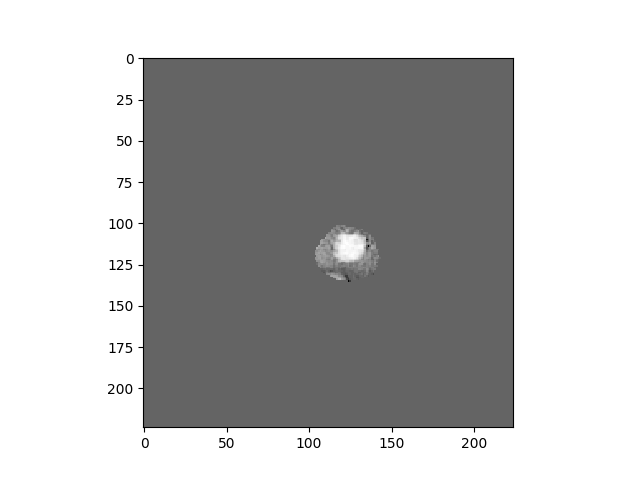
\includegraphics[width=200]{5_image_predict.png}
\end{center}

Pe ultimul set de date pe care s-a f\u{a}cut prezicerea se poate observa c\u{a} exist\u{a} aceea\c{s}i problem\u{a}, un ventricul st\^{a}ng mult mai mare detectat.

\par

Din imaginile ilustrate mai sus putem s\u{a} tragem o concluzie, aceea c\u{a}, re\c{t}eaua neuronal\u{a} face detec\c{t}ii a ventricului st\^{a}ng mult prea mari, \^{i}ns\u{a} sunt acceptabile pentru a trece la urm\u{a}torul pas, acela de a prezice volumul de s\^{a}nge care curge prin ventriculul st\^{a}ng. O posibil\u{a} modalitate de a for\c{t}a re\c{t}eaua neuronal\u{a} s\u{a} prezic\u{a} un ventricul st\^{a}ng mai mic ar fi s\u{a} supliment\u{a}m num\u{a}rul de imagine de antrenare cu inimi aflate la sistol\u{a}.

\section{Prezicerea volumului de s\^{a}nge}

Dup\u{a} antrenarea re\c{t}eleu neuronale pentru a segmenta ventriculul st\^{a}ng a inimii, putem trece la pasul de a prezice volumul de s\^{a}nge care curge prin inim\u{a}.

\par

Primul pas \^{i}n realizarea acestui lucru este de a citi datele salvate din fi\c{s}ierul CSV, date pe care le-am salvat din metadatele de la fi\c{s}ierele DICOM aferent fiecarui pacient. Dup\u{a} citim fiecare imagine PNG care provine de la un pacient, \^{i}ns\u{a} din cauza faptului c\u{a} fiecare imagine are o dimensiune de [256 x 256] iar re\c{t}eaua neuronal\u{a} care face segmentarea ventricului st\^{a}ng accept\u{a} doar imagine de dimensiunea [224 x 224] vom fi nevoi\c{t}i s\u{a} mai t\u{a}iem din fiecare imagine c\^{a}te 32 de pixeli pe orizontal\u{a} \c{s}i vertical\u{a} ca s\u{a} \^{i}i aducem la dimensiunea corespunz\u{a}toare.

\par

Al doilea pas \^{i}l presupune trecerea imaginilor, ale unui pacient, prin re\c{t}eaua neuronal\u{a}, pentru a se segmenta ventriculul st\^{a}ng al inimii. \^{I}nainte de a introduce imaginile \^{i}n re\c{t}eaua neuronal\u{a}, acestea trebuiesc normalizate \c{s}i centrate la zero. Dup\u{a} introducerea imaginilor \^{i}n re\c{t}eaua neuronal\u{a} \c{s}i ob\c{t}inerea rezultatelor, acestea sunt salvate sub format PNG \^{i}ntr-un fi\c{s}ier.

\par

Al treilea pas \^{i}l presupune num\u{a}rarea pixelilor care fac parte din ventriculul st\^{a}ng al inimii \c{s}i salvarea acestor valori pentru pa\c{s}ii urm\u{a}tori.

\par 

Al patrulea pas, \c{s}i ultimul din aceast\u{a} faz\u{a}, este calcularea efectiva a cantit\u{a}\c{t}ii de s\^{a}nge care curge prin ventriculul st\^{a}ng la momentul respectiv. Prima dat\u{a} se va stabilii care frame apar\c{t}ine sistolei \c{s}i care apar\c{t}ine diastolei, aces lucur se va face cu ajutorul numarului de pixeli detecteta\c{t}i de re\c{t}eaua neuronal\u{a}, astfel \^{i}nc\^{a}t frame-ul cu cei mai pu\c{t}ini pixeli va fi atribuit  sistolei, iar frame-ul cu cei mai mul\c{t}i pixeli va fi atribuit diastolei. Dup\u{a} determinarea frame-urilor care apar\c{t}ine siastolei si diastolei se poate calcula volumul de s\^{a}nge la siastol\u{a} \c{s}i la diastol\u{a}. Se iau toate pozele care apar\c{t}in respectivelor frame-uri iar numarul de pixeli pe care \^{i}l au se \^{i}nmul\c{t}este cu distan\c{t}a dintre ele, iar rezultatul ob\c{t}inut reprezint\u{a} volumul de s\^{a}nge care curge la diastol\u{a}, respectiv sistol\u{a}, \^{i}n fram-ul respectiv. Pentru a calcula volumul total care curge \^{i}n toate fram-urile vom proceda \^{i}n felul urm\u{a}tor, vom lua pentru fiecare frame ( \^{i}l vom nota cu $f$ ) fram-ul din fa\c{t}a lui (\^{i}l vom nota cu $f_v$ ) \c{s}i distan\c{t}a dintre ele (\^{i}l vom nota cu $\Delta$ ) \c{s}i vom aplica urm\u{a}toare formul\u{a}:

$$ V = \frac{1}{1000} \sum_i \Delta_i \frac{f_i + \sqrt{f_i * f_{v_i}} + f_{v_i}}{3} $$

Valoarea 1000 care apare \^{i}n fa\c{t}a formulei este un parametru pus din cauz\u{a} c\u{a} de cele mai multe ori calculul volumului de s\^{a}nge ie\c{s}ea de cele mai multe ori mult prea mare de c\^{a}t ar fi trebuit, din aceast\u{a} cauz\u{a} a fost ad\u{a}ugat \^{i}n formul\u{a}.

\par

Rezultatele ob\c{t}inute la pasul patru vor fi salvate intr-un fi\c{s}ier CSV. De precizat faptul c\u{a} acestea nu sunt valorile finale \c{s}i nu vom calcula la acest pas frac\c{t}ia de ejec\c{t}ie a inimii deoarece, a\c{s}a cum am vazut \c{s}i \^{i}n capitolul anterior, re\c{t}eaua noastr\u{a} neuronal\u{a} nu face preziceri tocmai perfect \c{s}i din acest\u{a} cauz\u{a} vom mai face o calibrare a datelor calculate, astfel \^{i}nc\^{a}t acestea s\u{a} fiu c\^{a}t mai aproape de adev\u{a}r.

\section{Calibrarea datelor}

Pentru a face partea de calibrare a datelor prezise de re\c{t}eaua neuronal\u{a} pentru volum de s\^{a}nge care curge la sistol\u{a} \c{s}i diastol\u{a} ne vom folosii de restul datelor pe care le oferea fi\c{s}ierele DICOM (num\u{a}rul de linii, numarul de coloane pe care le are o radiografie, spa\c{t}iul dintre frame-uri, grosimea radiografiei, v\^{a}rsta pacientului, unghiul din care a fost f\u{a}cut\u{a} radiografia) pe l\^{a}ng\u{a} acestea vom mai ad\u{a}uga \c{s}i valorile calculate pe baza prezicerilor f\u{a}cute de re\c{t}eaua neuronal\u{a} pentru sistol\u{a} \c{s}i diastol\u{a}. Cu ajutorul acestor date vom folosii algoritmul \textbf{\textit{Gradient Bootstrap}} pentru a prezice diferen\c{t}a dintre valorile reale la sistol\u{a} \c{s}i diastol\u{a} \c{s}i valorile prezise.

\par

Pentru algoritmul \textbf{\textit{Gradient Bootstrap}} vom folosii ca date de antrenare pacien\c{t}ii pentru care \c{s}tiim valorile adev\u{a}rate la sistol\u{a} \c{s}i diastol\u{a} ( sunt 700 de pacienti din 1140 pentru care s\c{t}iim valorile reale la sistol\u{a} \c{s}i diastol\u{a} ) iar pentru ceilal\c{t}i pacien\c{t}i vom prezice aceste dou\u{a} valori.

\par

\textbf{\textit{Gradient Bootstrap}} este un algoritm de Machine Learning folosit pentru probleme de regresii \c{s}i clasificare. Acesta se folose\c{s}te de un arbore de decizii pe care \^{i}l construie\c{s}te ca s\u{a} minimizeze funnc\c{t}ia de pierdere, unde func\c{t}ia de pierdere reprezint\u{a} diferen\c{t}a la p\u{a}trat dintre prezicerea f\u{a}cut\u{a} \c{s}i prezicerea f\u{a}cut\u{a} de c\u{a}tre algoritm.

$$ f = (y - y_p )^2 $$

Fiecare prezicerea nou\u{a} este f\u{a}cut\u{a} pe baza prezicerilor anterioare, astfle \^{i}nc\^{a}t fiecare nou nivel este consturit ca s\u{a} minimizeze func\c{t}ia de cost al nivelului anterior.

\begin{center}
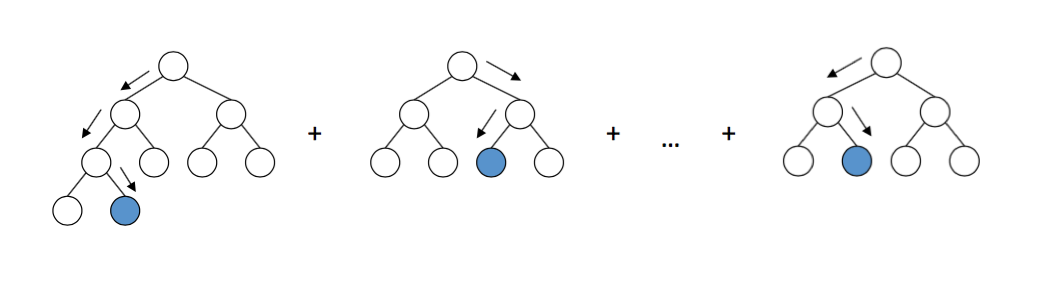
\includegraphics[width=400]{gradinet_boosting.png}
\end{center} 

Pentru algoritmul \textbf{\textit{Gradient Bootstrap}} am ales urm\u{a}torii parametrii pentru a se efectua partea de regresie \^{i}n prezicerea diferen\c{t}elor dintre sistol\u{a}, respectiv diastol\u{a}, a valorilor reale cu valorile calculate la pacien\c{t}ii pentru care nu \c{s}tiim valorile reale la sistol\u{a} \c{s}i diastol\u{a}. Ca rat\u{a} de \^{i}nv\u{a}\c{t}are am ajuns \^{i}n urma experimentelor la valoarea 0.001, acesta fiind \c{s}i cel mai greu parametru de setat. Ca num\u{a}r maxim de nivele am l\u{a}sat valorea 3, aceast\u{a} valoarea a fost aleas\u{a} pentru a prevenii efectul de overfitting, iar numarul minim de frunze la un nod a fost lasat la valoarea 2, iar num\u{a}rul maxim de estimatori a fost setat la 2500, tot din motivul de a se prevenii efectul de overfitting.

\par

Dup\u{a} aflarea valorilor prezise de c\u{a}tre algoritm putem calcula noile preziceri pentru sistol\u{a} \c{s}i diastol\u{a}, acestea vor reprezenta diferen\c{t}a dintre valorea calculat\u{a} pe baza prezicerilor f\u{a}cute de c\u{a}tre re\c{t}eaua neuronal\u{a} \c{s}i eroarea dintre valoarea prezis\u{a} \c{s}i valoarea adev\u{a}rat\u{a} pe care algoritmul \^{i}l indic\u{a}. 

\par

Valorile rezultate \^{i}n urma calculelor de mai sus reprezint\u{a} valorile finale pentru cantitatea de s\^{a}nge care curge la sistol\u{a} \c{s}i la diastol\u{a}, prin urmare acum se poate calcula frac\c{t}ia de ejec\c{t}ie, pe care o vom definii \^{i}n felul urm\u{a}tor:

$$ E_j = 100 * \frac{V_D - V_S}{V_D} $$

Unde $V_D$ reprezint\u{a} volumul de s\^{a}nge care curge la diastol\u{a}, iar $V_S$ reprezint\u{a} volumul de s\^{a}nge care curge la sistol\u{a} iar rezultatul final este reprezentat \^{i}n procent cu valori \^{i}ntre 0 \c{s}i 100. \^{I}n urma valorii rezultate se poate determina dac\u{a} un pacient are probleme cu inima \c{s}i c\^{a}t de grav este aceast\u{a} sau dac\u{a} este s\u{a}n\u{a}tos. Astfel c\u{a}, dac\u{a} frac\c{t}ia de ejec\c{t}ie este mai mare de 75\% atunci pacientul este declarat bolnav \c{s}i este hiperdinamic, dac\u{a} este \^{i}ntre 55\% \c{s}i 75\% atunci pacientul este declarat s\u{a}n\u{a}tos, dac\u{a} este 45\% \c{s}i 54\% atunci pacientul este declarat bolnav av\^{a}nd o frac\c{t}ie de ejec\c{t}ie u\c{s}or anormal\u{a}, dac\u{a} este \^{i}ntre 35\% \c{s}i 44\% atunci pacientul este delcarat bolnav cu o frac\c{t}ie de ejec\c{t}ie moderat anormal\u{a}, iar daca este sub 35\% atunci pacientul este bolnav cu o frac\c{t}ie de ejec\c{t}ie sever anormal\u{a}.

\section{Rezultate}

\^{I}n tabelul de mai jos sun prezentate c\^{a}teva example de rezultate ob\c{t}inute la pacien\c{t}ii pentru care nu se \c{s}tiau valorile reale a sistolei \c{s}i diastolei de la \^{i}nceput, de asemenea sunt ar\u{a}tate \c{s}i valorile lor reale pentru a putea fi comparate cu rezultatele ob\c{t}inute \c{s}i sunt calculate frac\c{t}iile de ejec\c{t}ie pentru valorile prezise \c{s}i valorile reale.

\begin{center}
 \begin{longtable}{|p{0.5cm}|p{2cm}|p{2cm}|p{2cm}|p{2cm}|p{2cm}|p{2cm}|} 
 \hline
 Nr. & Diastola real\u{a} & Diastola prezis\u{a} & Sistola real\u{a} & Sistola prezis\u{a} & Frac\c{t}ia de ejec\c{t}ie pentru valorile reale & Frac\c{t}ia de ejec\c{t}ie pentru valorile prezise  \\ [0.5ex] 
 \hline\hline
 1 &  158.0 & 158.7 & 76.0 & 63.61 & 51,8\% & 59,9\% \\
 \hline
 2 &  44.2 & 35.69 & 15.6 & 12.94 & 64,7\% & 63,7\% \\ 
 \hline
 3 &  129.7 & 128.44 & 83.2 & 38.6 & 35,8\% & 69,9\% \\
 \hline
 4 &  121.1 & 126.34 & 39.2 & 53.79 & 67,3\% & 57,4\% \\
 \hline
 5 &  127.4 & 145.78 & 57.8 & 57.99 & 54,63\% & 60,2\% \\
 \hline
 6 &  177.7 & 188.18 & 76.4 & 77.49 & 57\% & 58,8\% \\
 \hline
 7 &  277.6 & 186.16 & 133.5 & 74.88 & 51,9\% & 59,7\% \\
 \hline
 8 &  210.1 & 209.73 & 167.5 & 102.7 & 20,2\% & 51\% \\
 \hline
 9 &  230.1 & 193.51 & 91.4 & 91.53 & 60.2\% & 52,7\% \\
 \hline
 10 &  315.8 & 213.66 & 122.3 & 98.24 & 61,2\% & 54\% \\
 \hline
\end{longtable}
\end{center}

Dup\u{a} cum se poate vedea din tabelul de mai sus, metoda pe care am abordato \^{i}n acest\u{a} lucrare face unele preziceri destul de aproape de adev\u{a}r ( exemplele 2 \c{s}i 6) unde valorile diastolei \c{s}i sitolei prezie sunt destul de aproape de adev\u{a} astfel \^{i}nc\^{a}t ca frac\c{t}iile de ejec\c{t}ie s\u{a} ias\u{a} asem\u{a}n\u{a}toare. Mai sunt unele preziceri unde valorile diastolei sunt apropiate, \^{i}ns\u{a} din cauz\u{a} c\u{a} valorile sistolei difere \^{i}ntre ele, valorile frac\c{t}iei de ejec\c{t}ie ies la o diferen\c{t}\u{a} destul de mare \c{s}i din aceast\u{a} cauz\u{a} un pacient poate fi declarat bolnav sau s\u{a}n\u{a}tos din gre\c{s}eal\u{a} (exemplele 1, 3, 4 \c{s}i 8) sau invers, valorile sistoli s\u{a} fiu apropiate iar valorile diastolei s\u{a} au o diferen\c{t}\u{a} destul de mare \^{i}ntre el \c{s}i din aceast\u{a} cauz\u{a} s\u{a} diagnostic\u{a}m un pacient ca find s\u{a}n\u{a}tos sau bolnav ( exemplele 5 \c{s}i 9) sau cazul cel mai neprielnic, c\^{a}nd \c{s}i valorile sitolei \c{s}i diastolei prezise difer\u{a} foarte mult de valorile adev\u{a}rate \c{s}i din aceast\u{a} cauza iesi o diferen\c{t}\u{a} destul de mare \^{i}ntre cele dou\u{a} frac\c{t}ii de ejec\c{t}ie.
\chapter{Concluzii}

\^{I}n lucrarea de fa\c{t}\u{a} s-a prezentat o metod\u{a} automat\u{a} prin care se poate calcula \^{i}n aproximativ 5-10 secunde frac\c{t}ia de ejec\c{t}ie la un pacient cu ajutorul unei re\c{t}ele neuronale de tip convolu\c{t}ional\u{a}, iar pe baza acestui calcul s\u{a} se stabileasc\u{a} dac\u{a} pacientul respectiv are sau nu probleme cu inima. Acest lucru se poate face \c{s}i de c\u{a}tre un medic specialist, \^{i}ns\u{a} timpul de calculare a frac\c{t}iei de ejec\c{t}ie este de aproximativ 20 de minute. Se poate trage concluzia c\u{a} prin aceast\u{a} metod\u{a} se reduce semnificativ timpul pe care un pacient trebuie s\u{a} \^{i}l a\c{s}tepte ca s\u{a} primesc\u{a} rezultatul de la medic \c{s}i \^{i}n plus, medicul poate ac\c{t}iona mai repede pentru a ajuta pacien\c{t}ii bolnavi de inim\u{a}.

\par

Din p\u{a}cate aceast\u{a} metod\u{a} nu este tocmai perfect\u{a}, a\c{s}a cum am vazut mai sus. Din aceast\u{a} cauz\u{a} unii pacien\c{t}i pot fi diagnostica\c{t}i ca fiind bolnavi, dar \^{i}n realitate nu au nimic, sau invers s\u{a} fie diagnostica\c{t}i ca fiind s\u{a}n\u{a}to\c{s}i dar de fapt ei au probleme cu inima. O mare problem\u{a} pe care o prezint\u{a} metoda abordat\u{a} \^{i}n lucrarea de fa\c{t}\u{a} este aceea c\u{a}, re\c{t}eaua neuronal\u{a} prezice de cele mai multe ori un ventricul st\^{a}ng mult prea mare dec\^{a}t este \^{i}n realitate, acest lucru dator\^{a}ndu-se faptului c\u{a} exist\u{a} \^{i}n exemplele de antrenare mai multe ventricule st\^{a}ngi aflate la diastol\u{a} dec\^{a}t la sistol\u{a}. O solu\c{t}ie pentru acest lucru ar fi s\u{a} se multiplice num\u{a}rul de imagini de antrenare c\^{a}nd inima se afl\u{a} la sistol\u{a}. O alt\u{a} solu\c{t}ie demn\u{a} de luat \^{i}n seam\u{a} este aceea de a se folosi un alt tip de re\c{t}ea neuronal\u{a} pentru detectarea ventricului st\^{a}ng. Cea mai bun\u{a} arhitectur\u{a} la ora actual\u{a} pentru acest lucru este cea dezvoltat\u{a} de c\u{a}tre Olaf Ronneberger, Philipp Fischer \c{s}i Thomas Brox de la Universitatea din Freiburg, Germania, botezat\u{a} U-net \cite{Unet}. S-a \^{i}ncercat implementarea unei arhitecturi similare la re\c{t}eaua neuronal\u{a}, \^{i}ns\u{a} nu am ob\c{t}inut nici un rezultat, iar implementarea ei este destul de complicat\u{a}.

\par

\^{I}n concluzie, metoda propus\u{a} \^{i}n lucrarea de fa\c{t}\u{a} este func\c{t}ional\u{a} \c{s}i \^{i}ntoarce rezultate de cele mai multe ori aproape de adev\u{a}r, fiind un punct de plecare destul de bun pentru implementarea unui sistem mult mai performant, care s\u{a} fie la fel de bun ca un medic specialist, \^{i}ns\u{a} mult mai rapid \^{i}n problema stabilirii dac\u{a} un pacient sufer\u{a} sau nu cu sistemul cardiac. 
\addtocontents{toc}{\vspace{2em}}
\setstretch{1.5}
\bibliographystyle{unsrtnat}
\begin{thebibliography}{9} 

\bibitem{knuthwebsite} 
Wikipedia, Rezonan\c{t}\u{a} Magnetic\u{a} Nuclear\u{a}
\\\texttt{https://ro.wikipedia.org/wiki/Rezonan\c{t}\u{a}\_magnetic\u{a}\_nuclear\u{a}}

\bibitem{knuthwebsite} 
Re\c{t}eaua Neuronal\u{a}
\\\texttt{https://ro.wikipedia.org/wiki/Re\c{t}ea\_neural\u{a}}

\bibitem{knuthwebsite} 
CS231n Convolutional Neural Networks for Visual Recognition
\\\texttt{http://cs231n.github.io}

\bibitem{knuthwebsite} 
Second Annual Data Science Bowl
\\\texttt{https://www.kaggle.com/c/second-annual-data-science-bowl}

\end{thebibliography}
\end{document}